\documentclass[11pt,a4paper]{article}

\usepackage[utf8]{inputenc}
\usepackage[T1]{fontenc}
\usepackage[spanish,es-nodecimaldot]{babel}
\usepackage{amsmath}
\usepackage{booktabs}
\usepackage{array}
\usepackage{geometry}
\usepackage{siunitx}
\usepackage{microtype}
\usepackage[hidelinks]{hyperref}
\usepackage{graphicx}
\geometry{margin=2.5cm}
\usepackage{subcaption}
\sisetup{
  output-decimal-marker = {,},
  round-mode = places,
  round-precision = 2
}

\title{Analisis ATCBR normalizacion}
\author{dani16595 }
\date{October 2026}

\begin{document}

\maketitle

\author{Daniel Muñoz}

\tableofcontents
\newpage

\section{Configuracion comun}
Todos los experimentos tienen esta misma configuracion comun

\begin{itemize}
    \item Número de agentes: $N=1000$.
    \item Número de pasos: $T=100000$.
    \item Velocidad de convergencia: $\mu=0.1$.
    \item Topología: grafo completo.
    \item Número de ejecuciones Monte Carlo por configuración: 100.
    \item Semilla maestra: 7.
\end{itemize}


\section{Validación del modelo ATBCR original}

El objetivo de este experimento es validar la implementación del modelo ATBCR original antes de introducir modificaciones sobre el dominio de opiniones o mecanismos de normalización. Esta validación sirve como \emph{baseline} para los experimentos posteriores del Paso 0.

En particular, se pretende comprobar si la implementación reproduce los principales regímenes descritos para el ATBCR original: extremización, fragmentación y consenso neutral. Para ello se estudia el efecto conjunto del umbral de confianza $\epsilon$ y del umbral de repulsión $\theta$.

\subsection{Configuración experimental}

Se utilizaron las mismas condiciones principales empleadas en el experimento ATBCR

\begin{itemize}
    \item Opiniones iniciales: distribución uniforme en $[0,1]$.
    \item Dominio de opiniones: $[0,1]$, aplicando el dominio original del ATBCR.
    \item Umbrales de confianza: $\epsilon\in\{0.2,0.3,0.4\}$.
    \item Umbrales de repulsión: $\theta\in\{0.7,0.8,0.9\}$.
\end{itemize}


\subsection{Métricas analizadas}

La proporción de agentes extremizados se calcula como el numero de agentes con valores mayores e iguales de 0.9 o menores e iguales de 0.1.

También se estudian las frecuencias acumuladas de las tres reglas del modelo:

\begin{align}
R_C &= \frac{N_C}{T},\\
R_N &= \frac{N_N}{T},\\
R_R &= \frac{N_R}{T},
\end{align}

donde $N_C$, $N_N$ y $N_R$ representan respectivamente el número de interacciones de confianza, inacción y repulsión. Por construcción,

\begin{equation}
R_C + R_N + R_R = 1.
\end{equation}

Finalmente, se utiliza la desviación estándar de las opiniones finales,

como medida de la dispersión final de la población.

\subsection{Resultados}

La Tabla~\ref{tab:baseline-results} resume los resultados obtenidos tras 100 ejecuciones independientes por configuración. Las frecuencias y la proporción de agentes extremizados se muestran en porcentaje.

\begin{table}[htbp]
\centering
\caption{Resultados finales del experimento}
\label{tab:baseline-results}
\small
\begin{tabular}{ccrrrrr}
\toprule
$\epsilon$ & $\theta$ &
$E$ (\%) &
IC95\% de $E$ &
$R_C$ (\%) &
$R_R$ (\%) &
$\sigma_X$ \\
\midrule
0.2 & 0.7 & 59.12 & [58.73, 59.50] & 33.77 & 17.25 & 0.3842 \\
0.2 & 0.8 & 39.99 & [39.58, 40.40] & 39.91 &  7.85 & 0.3160 \\
0.2 & 0.9 &  3.68 & [ 2.60,  4.75] & 43.88 &  0.29 & 0.2406 \\
0.3 & 0.7 & 59.86 & [59.35, 60.37] & 35.04 & 17.60 & 0.3865 \\
0.3 & 0.8 & 36.47 & [35.27, 37.66] & 48.14 &  6.43 & 0.3011 \\
0.3 & 0.9 &  0.08 & [ 0.05,  0.11] & 89.68 &  0.04 & 0.0125 \\
0.4 & 0.7 & 87.13 & [84.14, 90.12] & 49.45 & 28.31 & 0.4377 \\
0.4 & 0.8 &  1.14 & [ 1.02,  1.25] & 94.38 &  0.27 & 0.0505 \\
0.4 & 0.9 &  0.01 & [ 0.00,  0.02] & 97.41 &  0.02 & 0.0014 \\
\bottomrule
\end{tabular}
\end{table}

\subsubsection{Efecto del umbral de repulsión}

Para un valor fijo de $\epsilon$, el aumento de $\theta$ reduce de forma muy marcada la proporción final de agentes extremizados. Por ejemplo, para $\epsilon=0.2$, cuando $\theta$ aumenta de $0.7$ a $0.8$ y posteriormente a $0.9$.

\begin{equation}
59.12\% \rightarrow 39.99\% \rightarrow 3.68\%
\end{equation}


El mismo comportamiento es todavía más pronunciado para $\epsilon=0.4$:

\begin{equation}
87.13\% \rightarrow 1.14\% \rightarrow 0.01\%.
\end{equation}

Esta caída coincide con una reducción drástica de la frecuencia de repulsión. Para $\epsilon=0.4$, $R_R$ pasa de aproximadamente $28.31\%$ con $\theta=0.7$ a $0.27\%$ con $\theta=0.8$ y a $0.02\%$ con $\theta=0.9$.

Esto es coherente con la definición del modelo: al aumentar $\theta$, la condición

\begin{equation}
|x_i-x_j|>\theta
\end{equation}

es más difícil de satisfacer, por lo que disminuye el número de encuentros capaces de activar la regla de repulsión.

\subsection{Interacción entre confianza y repulsión}

El efecto de $\epsilon$ no puede interpretarse de manera aislada. En particular, para $\theta=0.7$, el incremento de $\epsilon$ no conduce a una reducción monotónica de la extremización:

\begin{equation}
59.12\% \rightarrow 59.86\% \rightarrow 87.13\%
\end{equation}

para $\epsilon=0.2$, $0.3$ y $0.4$, respectivamente.

El caso $(\epsilon,\theta)=(0.4,0.7)$ es especialmente relevante. En esta configuración coexisten una frecuencia elevada de confianza,

\begin{equation}
R_C \approx 49.45\%,
\end{equation}

y una frecuencia elevada de repulsión,

\begin{equation}
R_R \approx 28.31\%.
\end{equation}

Por tanto, un mayor umbral de confianza no implica necesariamente una menor extremización. La dinámica resulta de la interacción entre ambas reglas: la confianza puede formar grupos compactos mientras la repulsión entre grupos suficientemente alejados continúa desplazándolos hacia los extremos.

\subsection{Casos de la diagonal principal}

Los tres escenarios de la diagonal reproducen los comportamientos cualitativos destacados en el trabajo original:

\begin{description}
    \item[$(\epsilon,\theta)=(0.2,0.7)$:] se obtiene una elevada proporción de opiniones extremas ($59.12\%$) y una dispersión final alta ($\sigma_X=0.3842$), compatible con la coexistencia de un grupo neutral y grupos extremos.

    \item[$(\epsilon,\theta)=(0.3,0.8)$:] aparece un régimen intermedio, con un $36.47\%$ de agentes extremizados y $\sigma_X=0.3011$, en el que el grupo neutral tiene mayor peso y los extremos son menos numerosos.

    \item[$(\epsilon,\theta)=(0.4,0.9)$:] prácticamente desaparecen las opiniones extremas ($0.01\%$) y la dispersión final es casi nula ($\sigma_X=0.0014$), lo que indica consenso alrededor de una opinión neutral.
\end{description}

\subsection{Evidencia gráfica de los regímenes finales}

La Figura~\ref{fig:heatmap-extremizacion} representa el porcentaje medio de agentes con opiniones extremas en las nuevas diferentes umbrales.

\begin{figure}[htbp]
    \centering
    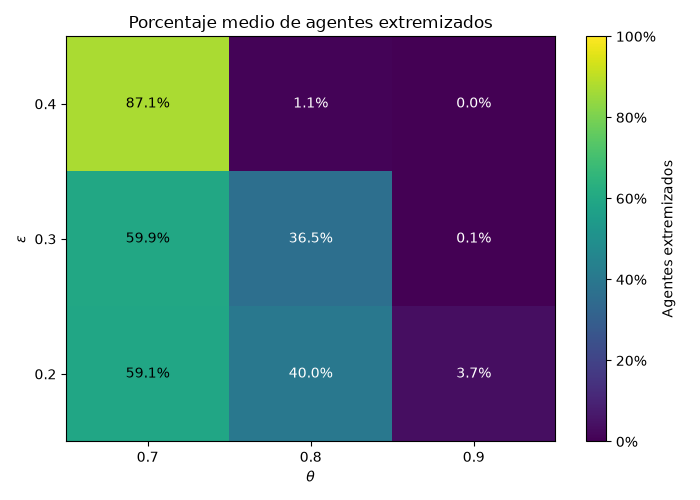
\includegraphics[width=0.72\textwidth]{imagenes/experimento_1/extremized.png}
    \caption{Porcentaje medio de agentes extremizados.}
    \label{fig:heatmap-extremizacion}
\end{figure}

La Figura~\ref{fig:distribuciones-finales} presenta las distribuciones agregadas de las opiniones finales. Los histogramas son una descripción de la forma de la distribución.

\begin{figure}[p]
    \centering
    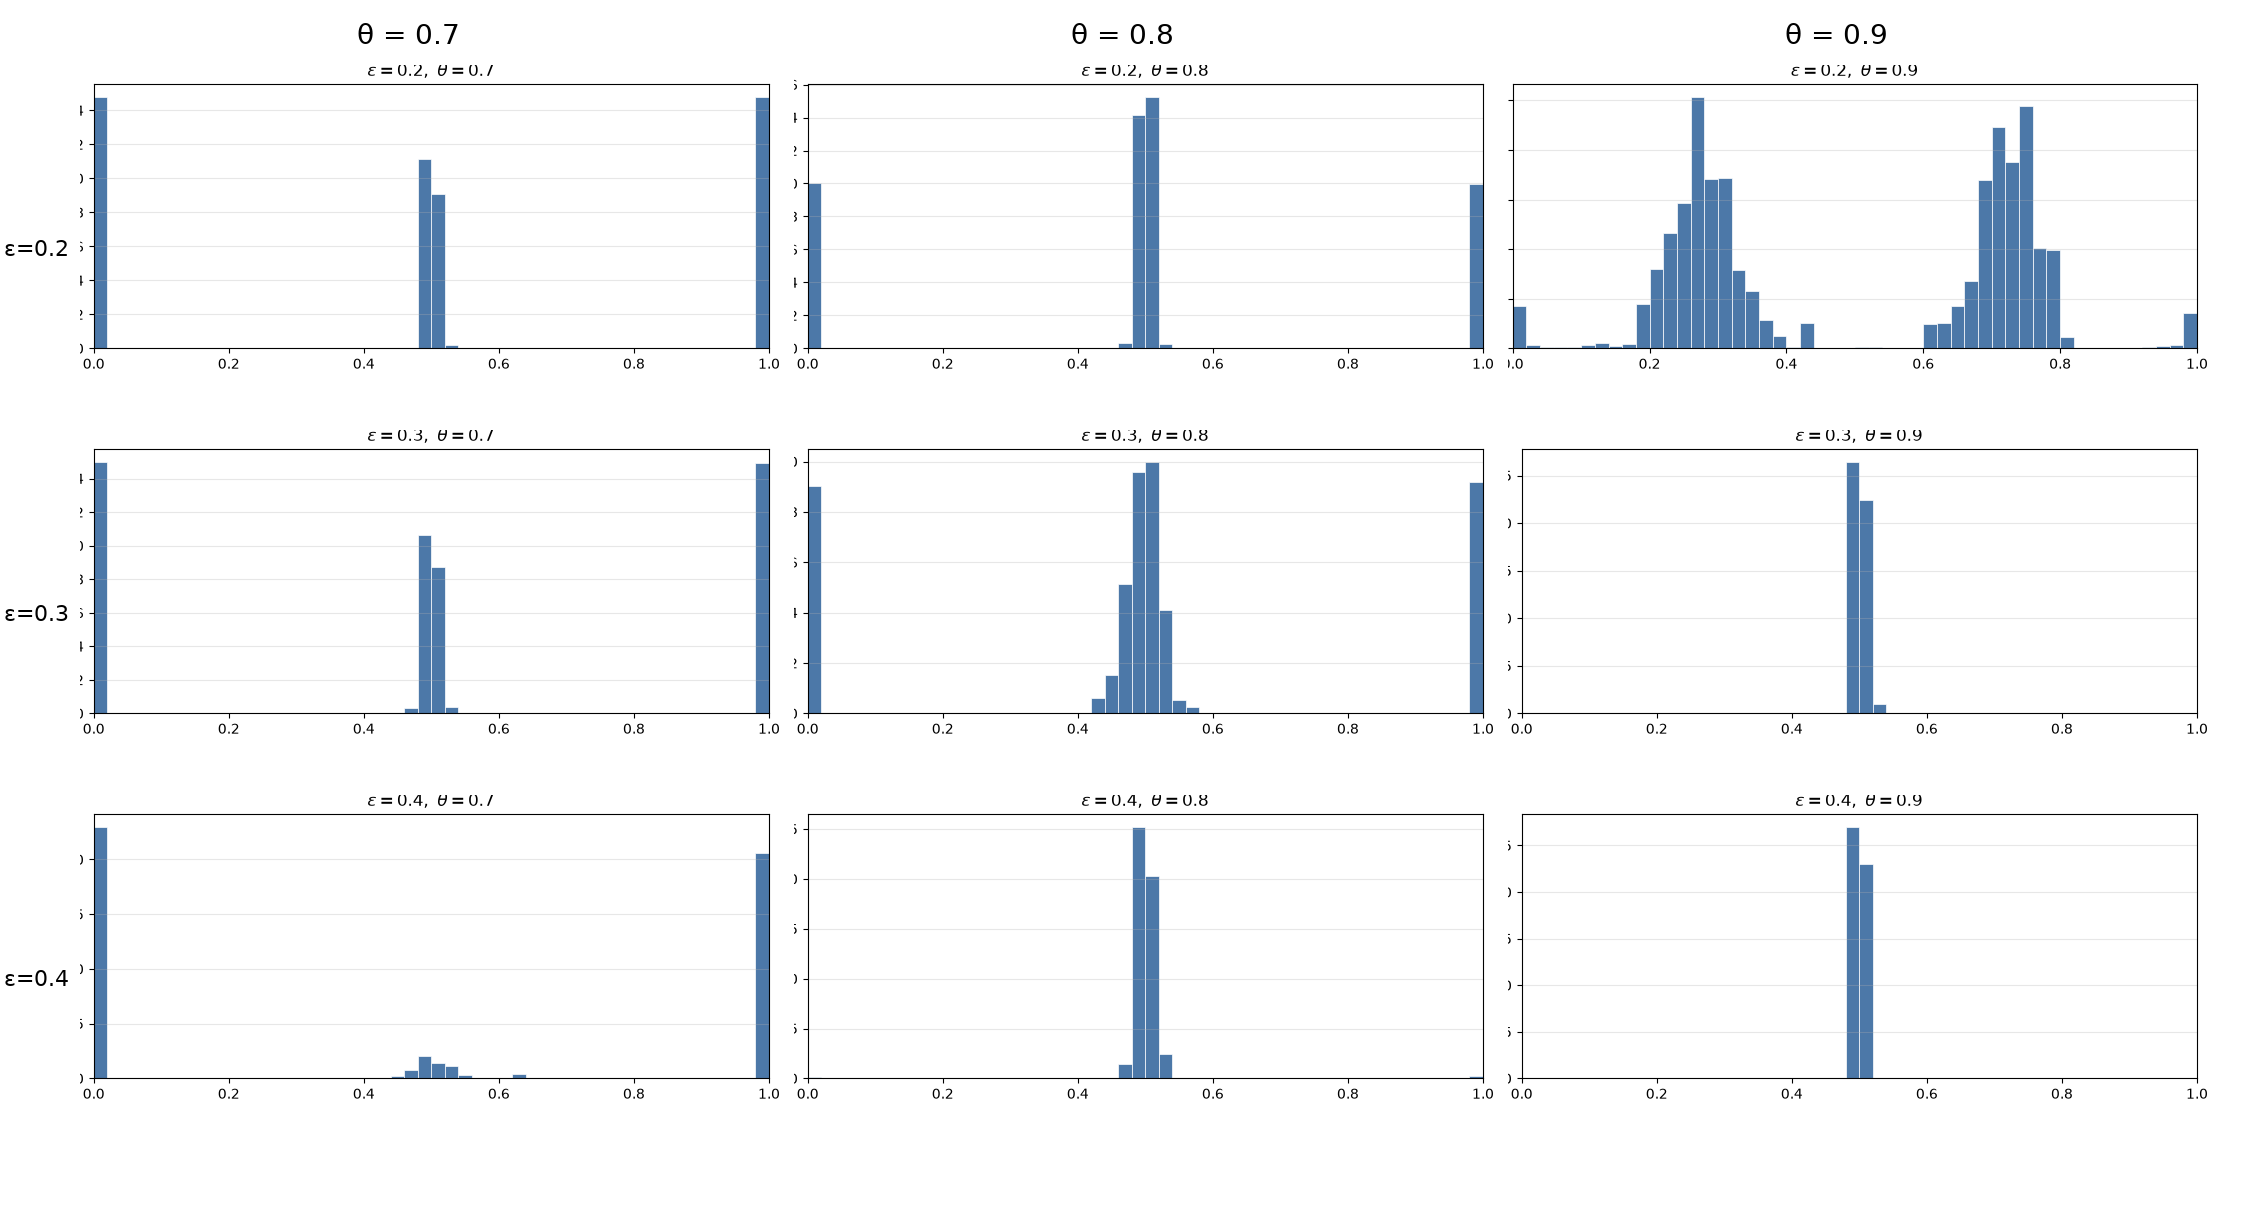
\includegraphics[width=\textwidth]{imagenes/experimento_1/final_distributions_3x3.png}
    \caption{Distribuciones agregadas de opinión final de las nueve configuraciones. Filas: umbral de confianza $\epsilon$; columnas: umbral de repulsión $\theta$. Cada panel reúne los últimos estados de $100$ réplicas de $1000$ agentes.}
    \label{fig:distribuciones-finales}
\end{figure}

Los casos $(0.2,0.7)$ y $(0.3,0.8)$ muestran concentraciones en los extremos y cerca de la región central, mientras que $(0.4,0.9)$ presenta una concentración muy marcada en torno a la opinión neutral. El caso $(0.2,0.9)$ exhibe dos concentraciones interiores en la distribución agregada.


\subsection{Representación gráfica de la evolución de la extremización}

La Figura~\ref{fig:evolucion-extremizacion} compara la evolución temporal de la proporción media de opiniones extremas. Permite distinguir regímenes de estabilización temprana de aquellos en los que la extremización continúa creciendo durante buena parte del horizonte experimental.

\begin{figure}[htbp]
    \centering
    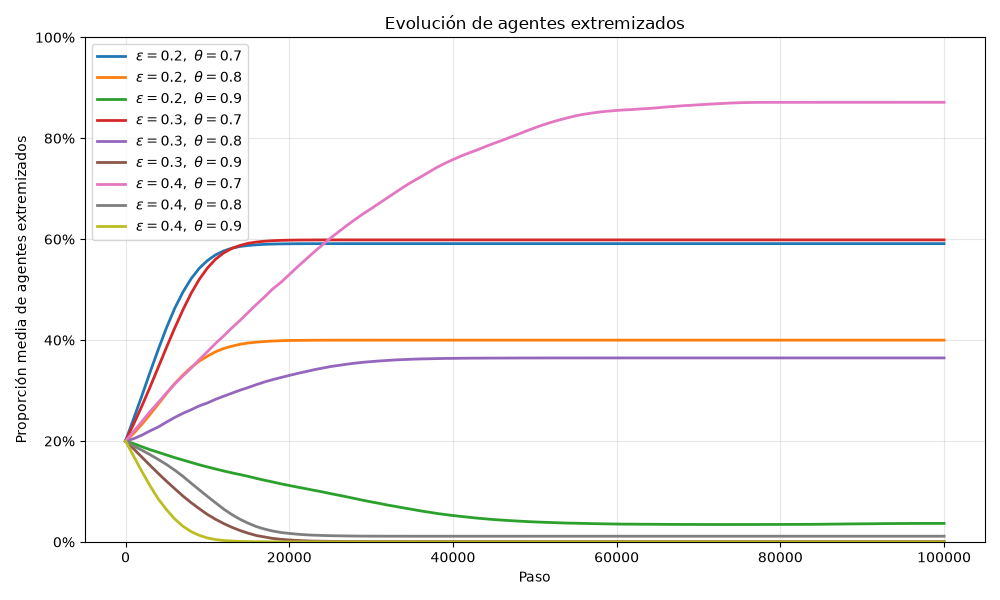
\includegraphics[width=\textwidth]{imagenes/experimento_1/extremized_comparison.png}
    \caption{Evolución temporal del porcentaje medio de agentes extremizados para las nueve combinaciones de umbrales.}
    \label{fig:evolucion-extremizacion}
\end{figure}


\subsection{Evolución temporal}

La Tabla~\ref{tab:temporal} presenta la evolución media de tres configuraciones representativas. $R_C^{(w)}$ y $R_R^{(w)}$ corresponden a las frecuencias locales calculadas en la ventana entre snapshots.

\begin{table}[htbp]
\centering
\caption{Evolución temporal media de configuraciones representativas.}
\label{tab:temporal}
\small
\begin{tabular}{ccrrrr}
\toprule
$(\epsilon,\theta)$ & $t$ &
$E$ (\%) &
$\sigma_X$ &
$R_C^{(w)}$ (\%) &
$R_R^{(w)}$ (\%) \\
\midrule
(0.2,0.7) & 10000  & 55.76 & 0.3801 & 30.75 & 17.31 \\
          & 20000  & 59.09 & 0.3864 & 33.85 & 17.42 \\
          & 50000  & 59.12 & 0.3843 & 34.10 & 17.60 \\
          & 80000  & 59.12 & 0.3842 & 34.36 & 17.63 \\
          & 100000 & 59.12 & 0.3842 & 34.16 & 17.56 \\
\midrule
(0.4,0.7) & 10000  & 37.71 & 0.3280 & 57.74 & 13.03 \\
          & 20000  & 52.97 & 0.3688 & 50.03 & 19.47 \\
          & 50000  & 82.08 & 0.4312 & 47.52 & 33.25 \\
          & 80000  & 87.12 & 0.4377 & 47.77 & 34.25 \\
          & 100000 & 87.13 & 0.4377 & 47.88 & 34.35 \\
\midrule
(0.4,0.9) & 10000  & 0.79 & 0.1597 & 90.40 & 0.001 \\
          & 20000  & 0.02 & 0.0315 & 99.97 & 0.000 \\
          & 50000  & 0.01 & 0.0015 & 99.97 & 0.000 \\
          & 80000  & 0.01 & 0.0014 & 99.98 & 0.000 \\
          & 100000 & 0.01 & 0.0014 & 99.98 & 0.000 \\
\bottomrule
\end{tabular}
\end{table}

La velocidad de estabilización depende claramente de la configuración. El escenario $(0.2,0.7)$ alcanza valores prácticamente estables alrededor de los $20000$--$50000$ pasos. En cambio, $(0.4,0.7)$ continúa incrementando de forma importante su grado de extremización después de $20000$ pasos, pasando de aproximadamente $52.97\%$ a $82.08\%$ entre $20000$ y $50000$ pasos, y no se estabiliza hasta aproximadamente $80000$ pasos.

Por otra parte, $(0.4,0.9)$ converge rápidamente hacia consenso: la desviación estándar disminuye de $0.1597$ en $t=10000$ a $0.0315$ en $t=20000$ y a aproximadamente $0.0015$ en $t=50000$. Durante esta evolución la repulsión local prácticamente desaparece y la confianza pasa a dominar la dinámica.

Estos resultados muestran que no existe un único horizonte corto que sea suficiente para todas las configuraciones. El uso de $T=100000$ permite observar adecuadamente tanto configuraciones de convergencia rápida como procesos de extremización más lentos.

\subsection{Conclusiones del experimento}

Los resultados obtenidos permiten considerar validada la implementación del ATBCR original como \emph{baseline} experimental. Se reproducen los principales regímenes cualitativos descritos en el trabajo original: extremización, fragmentación y consenso neutral.

El umbral de repulsión tiene un impacto especialmente acusado: al aumentar $\theta$, disminuye la frecuencia de activación de la regla de repulsión y, de forma asociada, disminuye la proporción final de opiniones extremas. Sin embargo, el efecto del umbral de confianza no es monotónico cuando se analiza de forma aislada, lo que confirma que el comportamiento del modelo emerge de la combinación de las reglas de confianza y repulsión.

Las 100 ejecuciones Monte Carlo muestran que las tendencias principales son robustas frente a la aleatoriedad, aunque algunos regímenes, especialmente $(0.4,0.7)$, presentan una variabilidad apreciable entre ejecuciones.

Finalmente, el análisis temporal confirma que $T=100000$ es un horizonte adecuado: algunas configuraciones estabilizan rápidamente, mientras que otras continúan evolucionando durante gran parte de la simulación. Esta validación proporciona una referencia fiable para los siguientes experimentos del Paso 0, en los que se modificará el dominio de opiniones y se analizarán mecanismos de normalización.

\section{Equivalencia del ATBCR entre los dominios [0,1] y [-1,1]}

El objetivo de este experimento es verificar que la transformación del espacio de opiniones original ([0,1]) al intervalo ([-1,1]) no modifica el comportamiento del modelo ATBCR, siempre que sus parámetros se adapten proporcionalmente.

Esta validación es necesaria para los experimentos posteriores, en los que se estudiará la eliminación del mecanismo de no superar rangos y la aplicación de estrategias de normalización sobre un espacio de opiniones centrado en cero.

\subsection{Configuración experimenta}

\begin{itemize}
    \item Opiniones iniciales: distribución uniforme en $[-1,1]$.
    \item Dominio de opiniones: $[-1,1]$, aplicando el clipping original del ATBCR.
    \item Umbrales de confianza: $\epsilon\in\{0.4,0.6,0.8\}$.
    \item Umbrales de repulsión: $\theta\in\{1.4,1.6,1.8\}$.
\end{itemize}

Sean $x_i(t)\in[0,1]$ las opiniones del modelo original. Se define la transformación afín
\begin{equation}
 y_i(t)=2x_i(t)-1, \qquad y_i(t)\in[-1,1].
\end{equation}
Para cualquier par de agentes,
\begin{equation}
 |y_i(t)-y_j(t)|=2|x_i(t)-x_j(t)|.
\end{equation}
Por tanto, para preservar las condiciones que activan las reglas de confianza, inacción y repulsión, se transforman los umbrales:
\begin{equation}
 \epsilon'=2\epsilon,\qquad \theta'=2\theta.
\end{equation}
Se mantiene el mismo coeficiente $\mu$, y el \emph{clipping} original a $[0,1]$ se transforma en \emph{clipping} a $[-1,1]$. Bajo la misma secuencia de encuentros y las condiciones iniciales correspondientes, esta transformación es equivalente paso a paso. Además, predice
\begin{equation}
 \sigma_Y(t)=2\sigma_X(t),
\end{equation}
puesto que $y_i-\bar y=2(x_i-\bar x)$. El desplazamiento de la media por sí solo no altera la desviación estándar: la duplicación procede del factor de escala.

\subsection{Resultados}
La Tabla~\ref{tab:resultados} muestra la fracción media de agentes extremizados (en porcentaje) y la desviación estándar media de las opiniones finales en cada dominio. Las proporciones de extremización son idénticas en las dos representaciones; las desviaciones estándar del dominio centrado son el doble de las originales.
\begin{table}[htbp]
\centering
\caption{Comparación de resultados agregados de los experimentos; medias de 100 réplicas por escenario.}
\label{tab:resultados}
\small
\begin{tabular}{ccrrrr}
\toprule
$\epsilon$ & $\theta$ & $E_{[0,1]}$ (\%) & $E_{[-1,1]}$ (\%) & $\overline{\sigma}_{[0,1]}$ & $\overline{\sigma}_{[-1,1]}$ \\
\midrule
0.2 & 0.7 & 59.11 & 59.11 & 0.384221 & 0.768441 \\
0.2 & 0.8 & 39.99 & 39.99 & 0.316027 & 0.632054 \\
0.2 & 0.9 & 3.68 & 3.68 & 0.240565 & 0.481131 \\
0.3 & 0.7 & 59.86 & 59.86 & 0.386528 & 0.773055 \\
0.3 & 0.8 & 36.47 & 36.47 & 0.301084 & 0.602169 \\
0.3 & 0.9 & 0.08 & 0.08 & 0.012495 & 0.024990 \\
0.4 & 0.7 & 87.13 & 87.13 & 0.437714 & 0.875428 \\
0.4 & 0.8 & 1.14 & 1.14 & 0.050503 & 0.101005 \\
0.4 & 0.9 & 0.01 & 0.01 & 0.001411 & 0.002821 \\
\bottomrule
\end{tabular}
\end{table}

La comparación de los dos experimentos confirma que las frecuencias de confianza, inacción y repulsión, coinciden en las nueve configuraciones. También coinciden las estadísticas de \texttt{extremized\_share} y \texttt{cluster\_count}. 

La igualdad de extremización responde a que los intervalos extremos $[0,0.1]\cup[0.9,1]$ se transforman exactamente en $[-1,-0.8]\cup[0.8,1]$.

\subsection{Equivalencia de trayectorias individuales}

Analizando la trayectoria de las opiniones teniendo en cuenta la comparacion entre los dos experimentos y usando la misma semilla, se ha demostrado que al final se llega a una opinion final que cumple esta funcion. siendo $x_i(t)$ la opinion del experimento 1.
\[
y_i(t) = 2x_i(t) - 1
\]


\subsection{Conclusiones}
Se ha obtenido que en los nueve escenarios tienen una equivalencia entre el ATBCR original en $[0,1]$ y su representación centrada en $[-1,1]$, siempre que se dupliquen los umbrales de confianza y repulsión. Las frecuencias de activación de reglas y la proporción de opiniones extremas permanecen invariantes, mientras que la desviación estándar se duplica como consecuencia de la transformación afín.

De este modo, el dominio $[-1,1]$ puede adoptarse como punto de partida para el experimento 0.3, donde la única modificación conceptual prevista será eliminar los limites del rango, sin alterar los umbrales efectivos ni las demás condiciones experimentales.



\section{ATBCR sin acotación de las opiniones}

El objetivo de este experimento es estudiar las consecuencias de eliminar la restricción de las opiniones al intervalo $[-1,1]$, sin aplicar ningún método de normalización. Se analiza la evolución y la dispersión de las opiniones, así como los cambios en la frecuencia de las reglas de confianza, inacción y repulsión.


\subsection{Configuración experimental}


\begin{itemize}
    \item Opiniones iniciales: distribución uniforme en $[-1,1]$.
    \item Dominio de opiniones: sin limites.
    \item Umbrales de confianza: $\epsilon\in\{0.4,0.6,0.8\}$.
    \item Umbrales de repulsión: $\theta\in\{1.4,1.6,1.8\}$.
\end{itemize}


\subsection{Crecimiento de las opiniones y dispersión}
Se observa un crecimiento de los valores de las opiniones a lo largo de los $100000$ pasos. En particular, aumentan el valor máximo absoluto, la magnitud absoluta media y la desviación estándar. Por lo que se observa no se limita exclusivamente a unos pocos agentes con valores extremos, sino que afecta a una fracción considerable de la población.

Para la configuración $(\epsilon,\theta)=(0.2,0.7)$, la media del máximo absoluto al final de las ejecuciones es aproximadamente $1.30\times10^{10}$. Estos resultados se muestra la ausencia de limites del dominio.

Conforme aumentan las diferencias entre opiniones y los umbrales permanecen fijos, las interacciones repulsivas adquieren progresivamente mayor importancia. En las nueve configuraciones estudiadas, la frecuencia media de repulsión en los ultimos pasos registrada alcanza el $100\,\text{\%}$, mientras que la frecuencia media de confianza es nula.

El tiempo necesario para alcanzar una frecuencia de repulsión superior al $99\,\text{\%}$ aumenta al elevar los umbrales. El efecto de $\theta$ parece más acusado que el de $\epsilon$.

\subsection{Influencia de los umbrales en el crecimiento}

Con el objetivo de analizar cómo afecta la eliminación del los limites a la dinámica entre agentes, se estudia la evolución temporal de las frecuencias de confianza y repulsión.

Se utilizan las frecuencias de repulsión y atracción calculadas sobre ventanas de $W=1000$ pasos.

La Figura~\ref{fig:exp03_frequencies} muestra la evolución de ambas frecuencias para distintas configuraciones de $\epsilon$ y $\theta$.

\begin{figure}[htbp]
    \centering
    \begin{subfigure}[b]{0.48\textwidth}
        \centering
        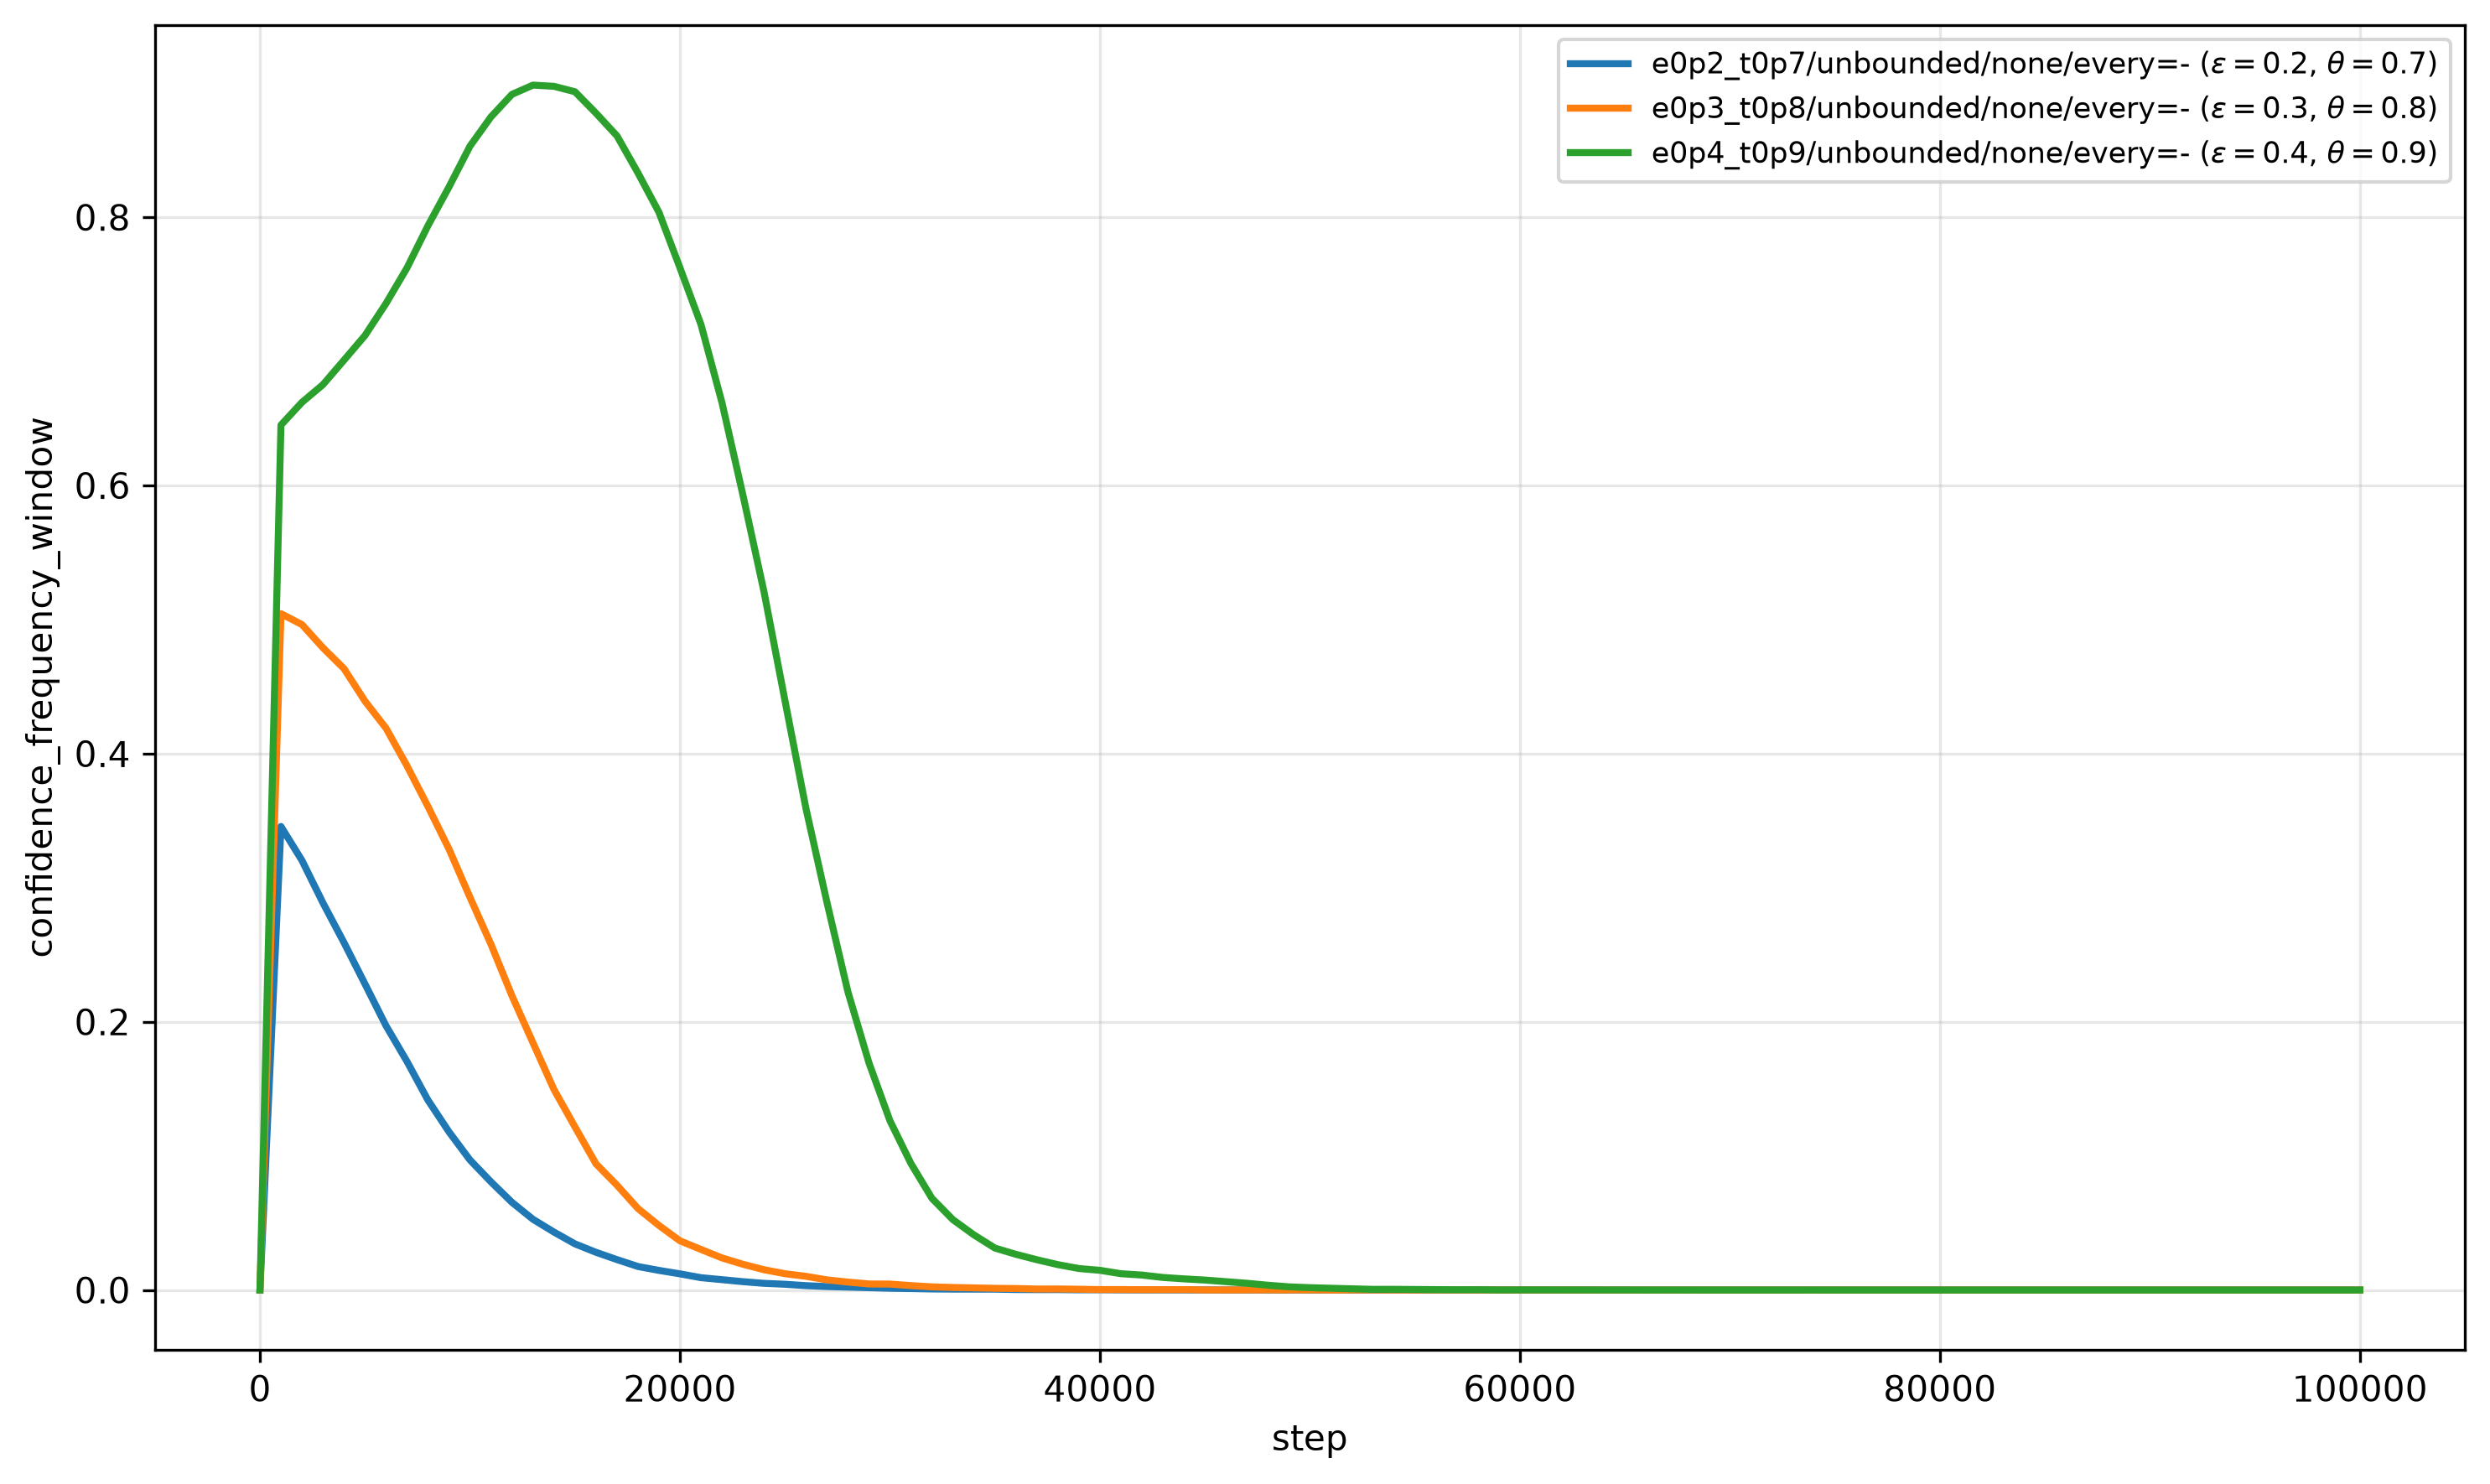
\includegraphics[width=\linewidth]{imagenes/experimento_3/confidence.png}
        \caption{Frecuencia de confianza.}
        \label{fig:exp03_confidence}
    \end{subfigure}
    \hfill
    \begin{subfigure}[b]{0.48\textwidth}
        \centering
        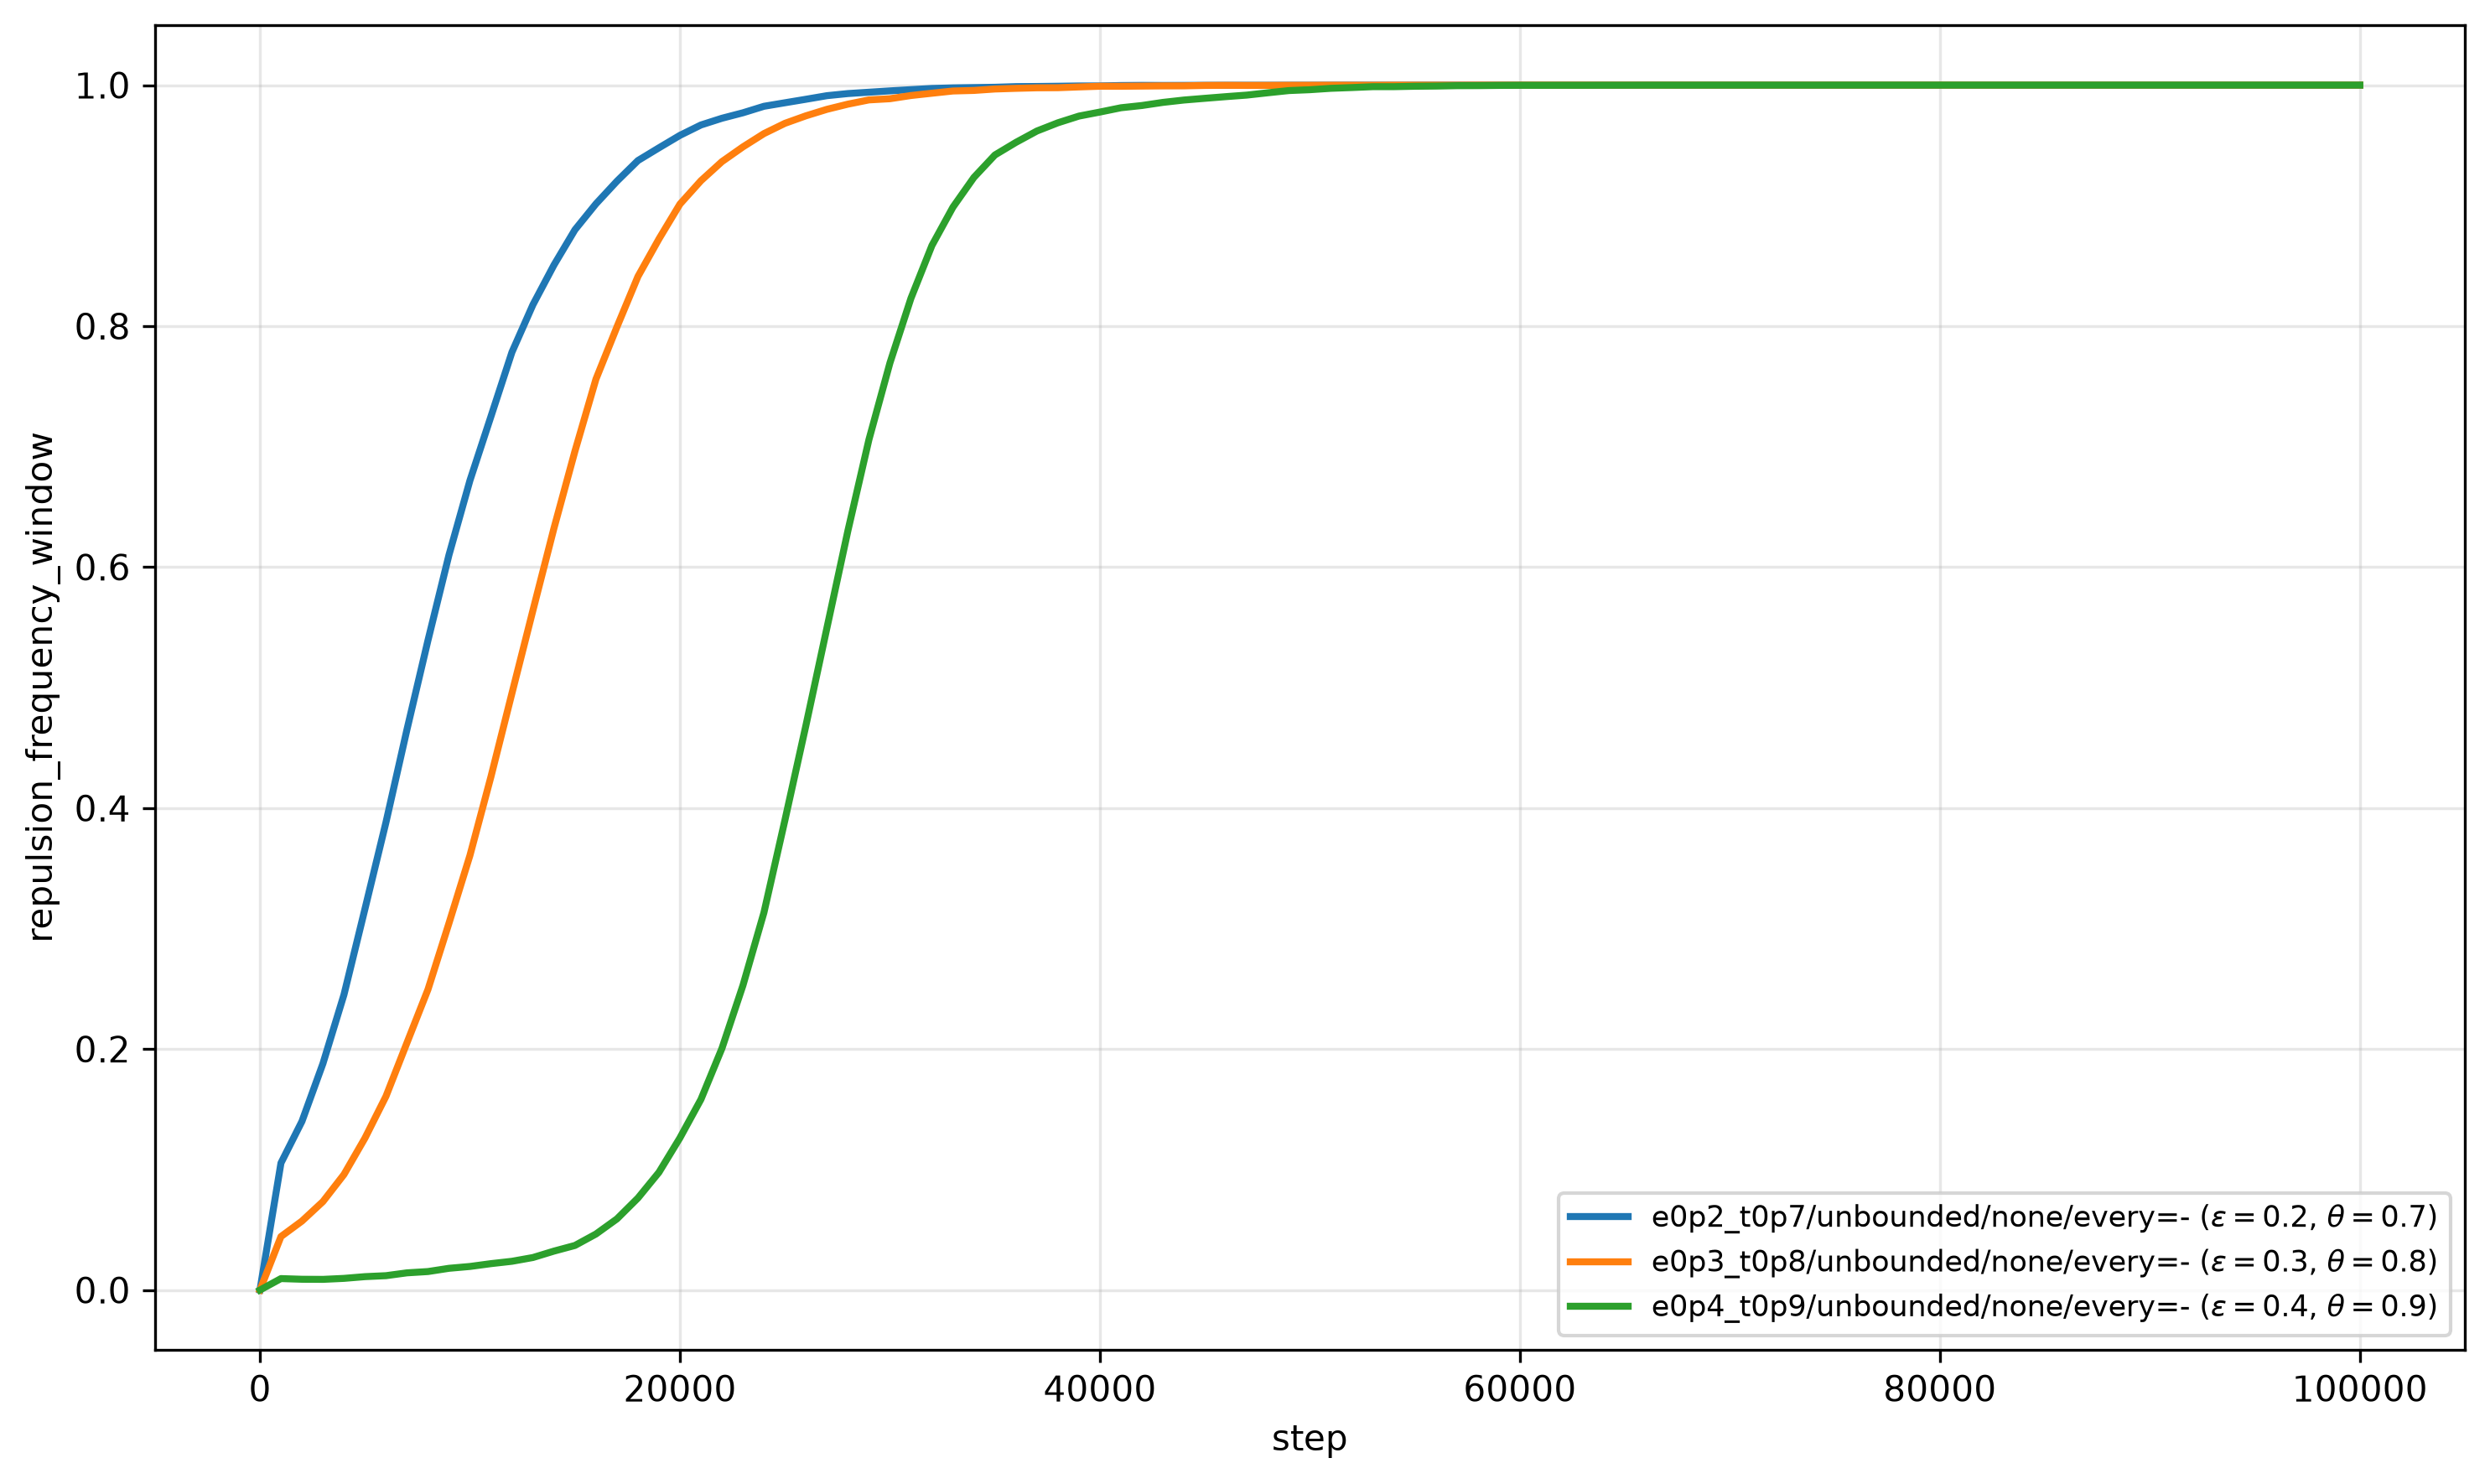
\includegraphics[width=\linewidth]{imagenes/experimento_3/repulsion.png}
        \caption{Frecuencia de repulsión.}
        \label{fig:exp03_repulsion}
    \end{subfigure}
    \caption{Evolución temporal de las frecuencias de confianza y repulsión del modelo ATBCR sin clipping, calculadas sobre ventanas de 1000 pasos.}
    \label{fig:exp03_frequencies}
\end{figure}


La Figura~\ref{fig:growth} compara tres configuraciones mediante la representación logarítmica de la opinion máxima absoluta. Las curvas son aproximadamente lineales durante una gran parte del periodo analizado, un comportamiento compatible con un crecimiento aproximadamente exponencial:

\begin{figure}[htbp]
\centering
    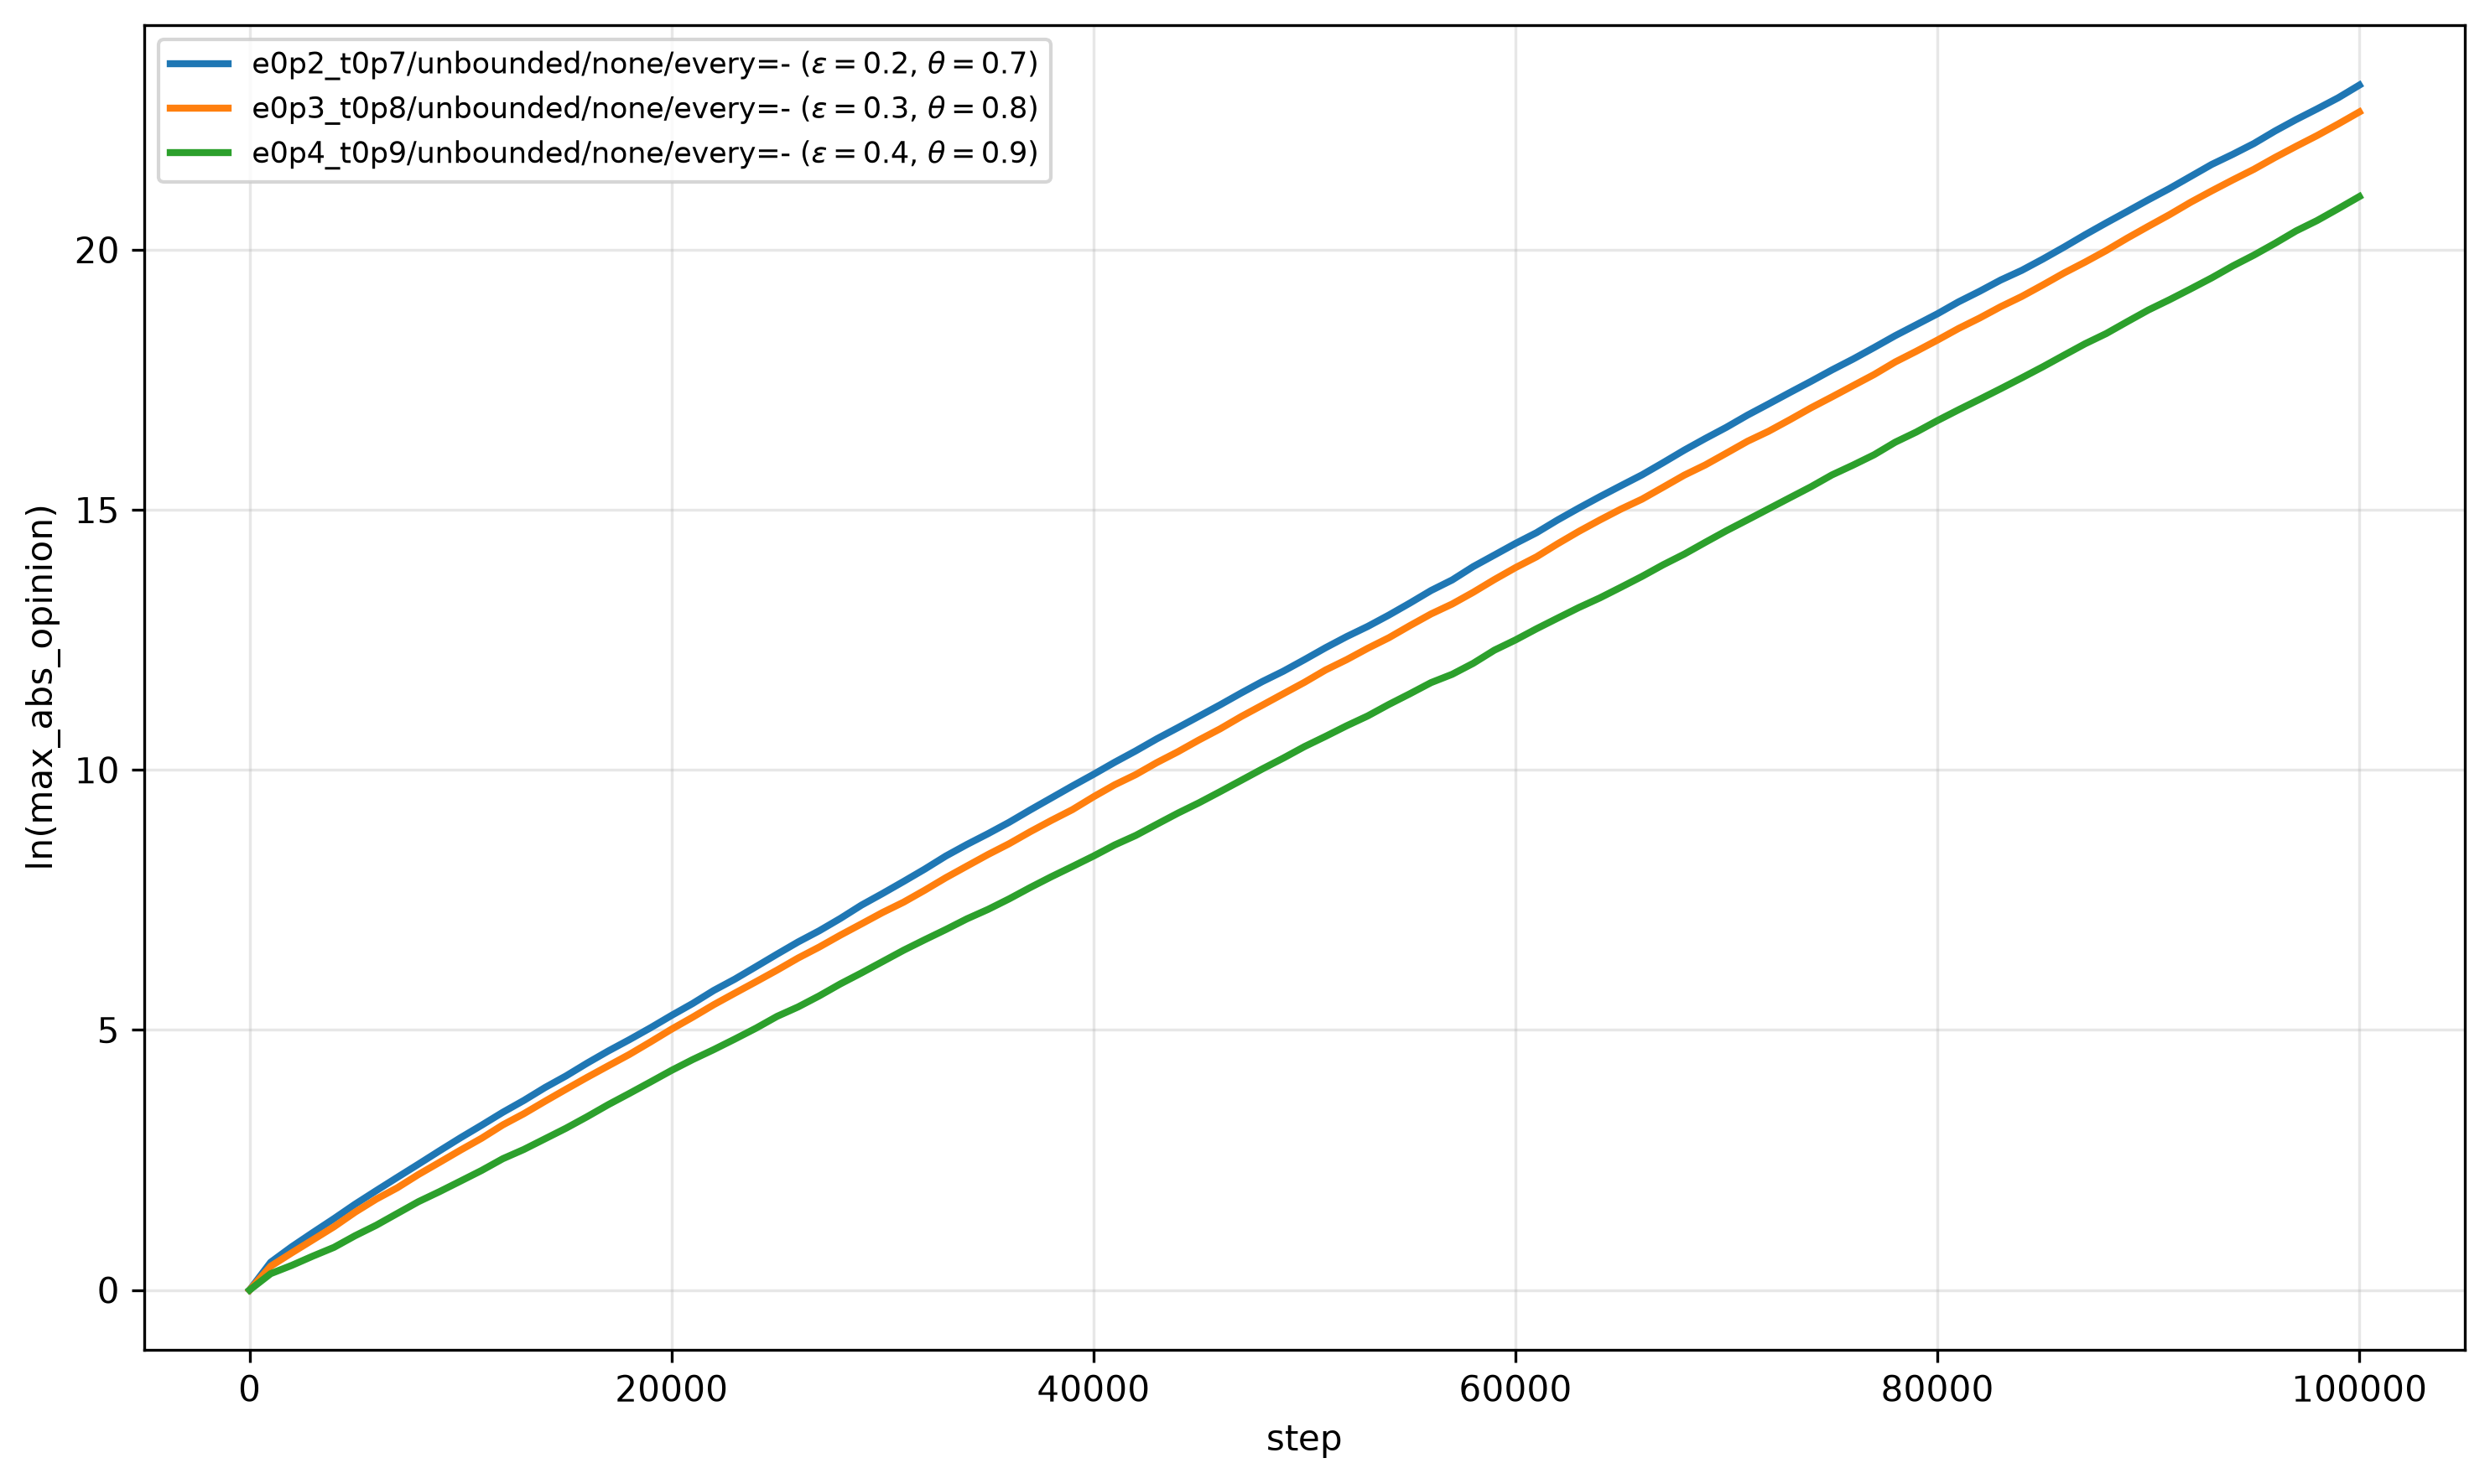
\includegraphics[width=\textwidth]{imagenes/experimento_3/growth.png}
\caption{Evolución temporal del logaritmo de la máxima absoluta de las opiniones, para tres configuraciones del modelo.}
\label{fig:growth}
\end{figure}

Visualmente, la configuración $(0.2,0.7)$ presenta una pendiente mayor que $(0.3,0.8)$, y esta mayor que $(0.4,0.9)$. Por tanto, los resultados sugieren que los umbrales no solo pueden retrasar hacia un dominio de repulsión, sino también influir en la tasa de crecimiento. Dado que en esta comparación $\epsilon$ y $\theta$ cambian simultáneamente.


\subsection{Conclusiones}
La eliminación de los limites, modifica la dinámica observada en el ATBCR acotado. En las nueve configuraciones experimentales analizadas, las opiniones y la dispersión de las opiniones aumentan, mientras que las interacciones de repulsión terminan dominando. La evolución es compatible con un crecimiento aproximadamente exponencial, cuya intensidad parece depender de los umbrales utilizados.

Estos resultados ponen de manifiesto que eliminar los límites del dominio puede favorecer a la separación entre opiniones y una pérdida de las interacciones de confianza.




\section{Normalización periódica mediante \texttt{max\_abs}}

\subsection{Objetivo y configuración}

En el experimento anterior, la eliminación del limite de opiniones permitió un crecimiento considerable de sus valores y favorece a las interacciones repulsivas. Este experimento estudia si una normalización periódica basada en el valor máximo, controla este crecimiento y cómo afecta a las interacciones y las distribuciones de opinión respecto al ATBCR acotado.

El operador de normalización aplicado a las opiniones $X(t)$ es
\begin{equation}
\displaystyle \frac{x_i(t)}{\max_j |x_j(t)|},\\[6pt]
\end{equation}

La normalización lo he aplicado cada $k\in\{10,100,1000,10000\}$ pasos. Entre aplicaciones se mantienen las reglas del ATBCR sin limites. Se estudian las nueve combinaciones de parámetros consideradas en los experimentos anteriores, con $N=1000$ agentes, $100\,000$ pasos y $100$ ejecuciones Monte Carlo por configuración. Las opiniones se inicializan en $[-1,1]$, empleando los umbrales correspondientes a ese dominio.

Se mantiene las proporciones entre las opiniones durante cada normalización, pero se modifica sus distancias absolutas:
\begin{equation}
\frac{|x_i-x_j|}{\max_l |x_l|}
\end{equation}

Por lo tanto, cuando la opinión máxima es mayor que uno, la normalización reduce las distancias entre agentes sin cambiar los umbrales de confianza y repulsión. Esto puede afectar a qué regla de interacción se activa después de normalizar. Si la magnitud máxima es menor que uno, la operación, por el contrario, amplía las distancias.

\subsection{Evolución de las frecuencias de interacción}

Se analizan las frecuencias de confianza y repulsión por ventanas de $W=1000$ pasos. Como en los casos anteriores.

\begin{figure}[htbp]
\centering
\begin{subfigure}[t]{0.48\textwidth}
  \centering
  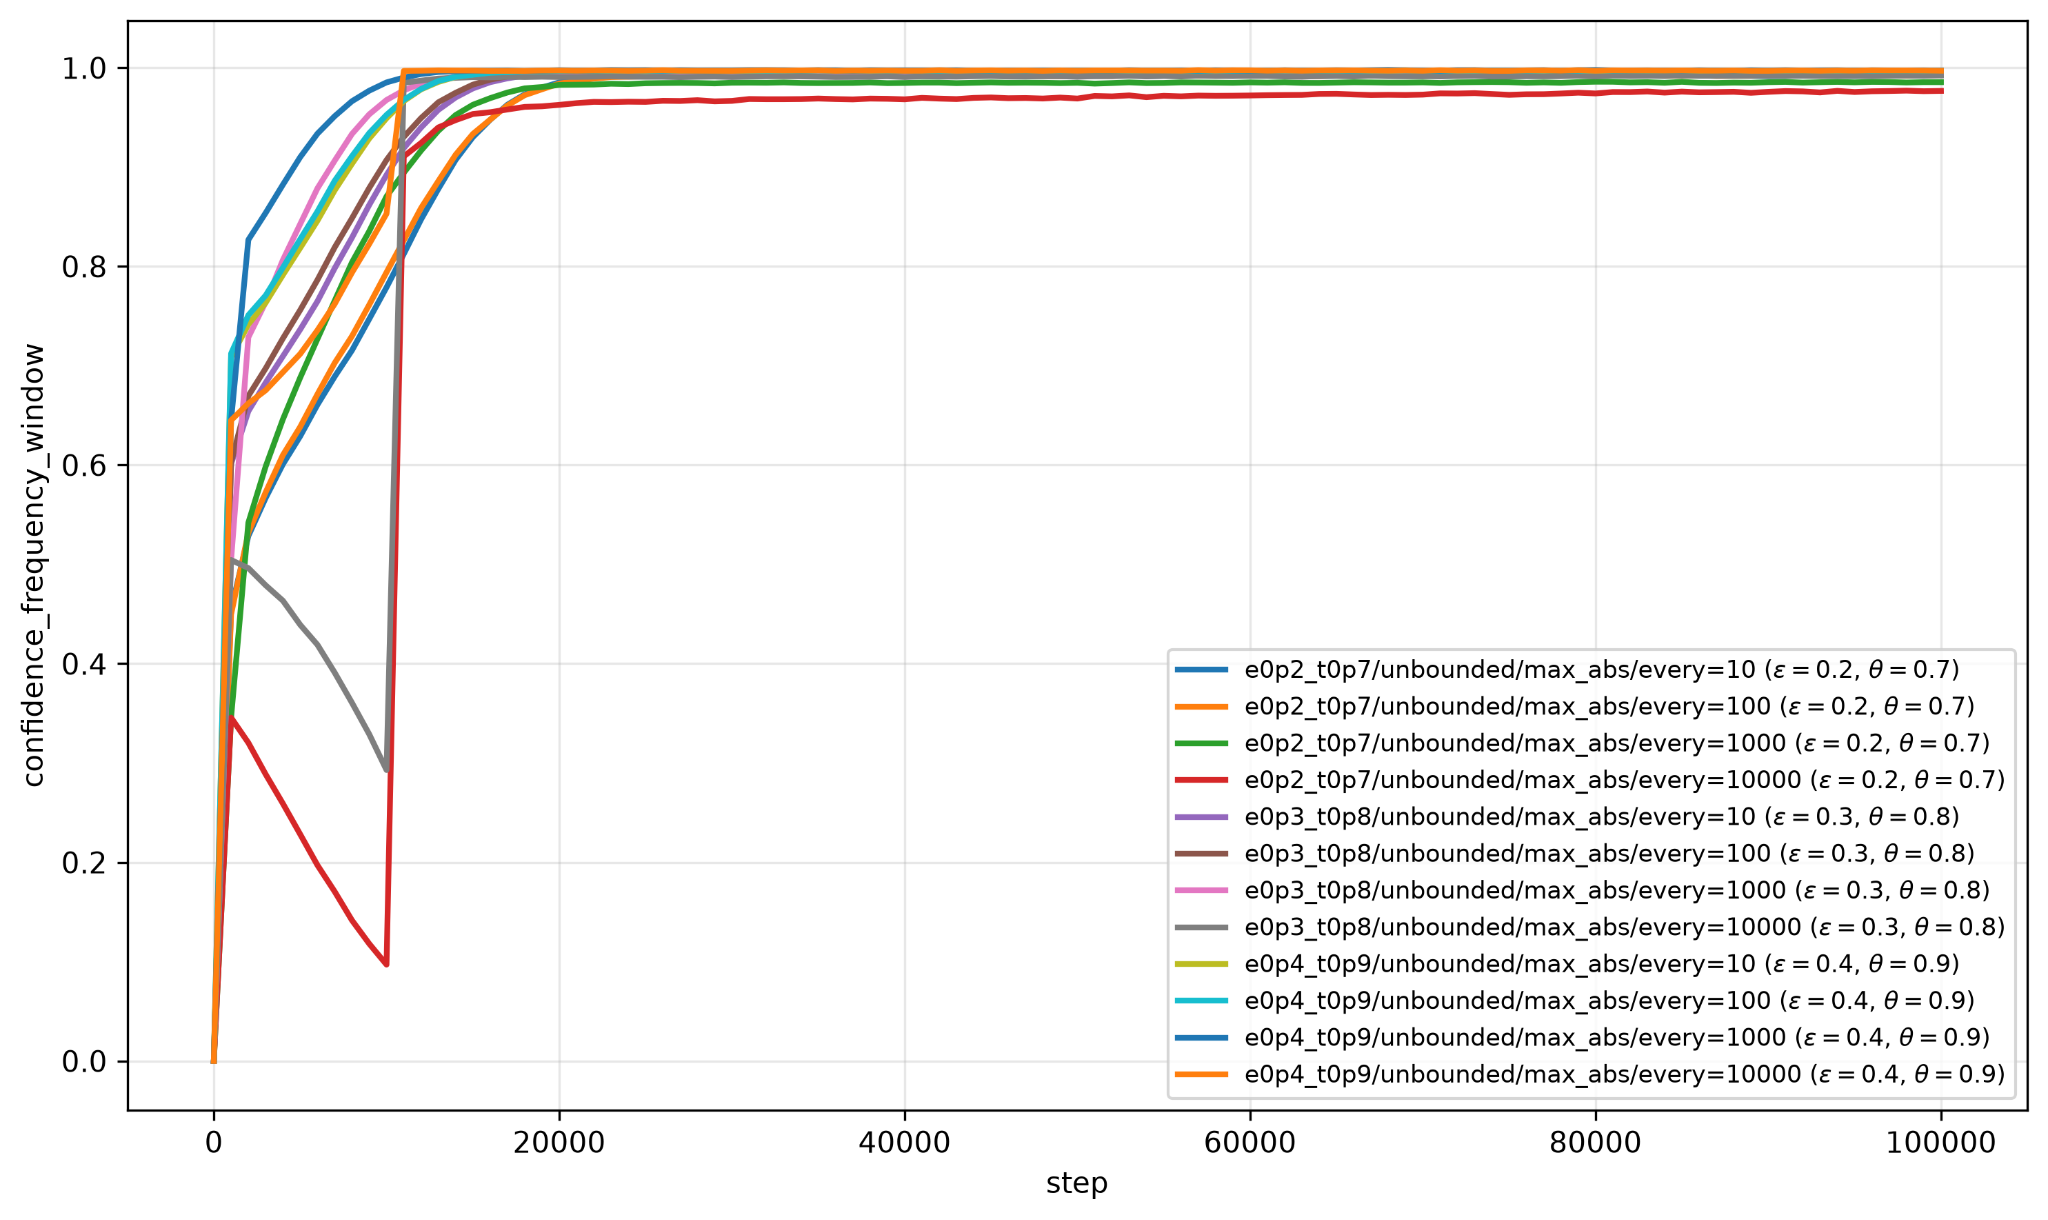
\includegraphics[width=\linewidth]{imagenes/experimento_4/confidence_window.png}
  \caption{Frecuencia de confianza.}
  \label{fig:exp04_confidence}
\end{subfigure}\hfill
\begin{subfigure}[t]{0.48\textwidth}
  \centering
  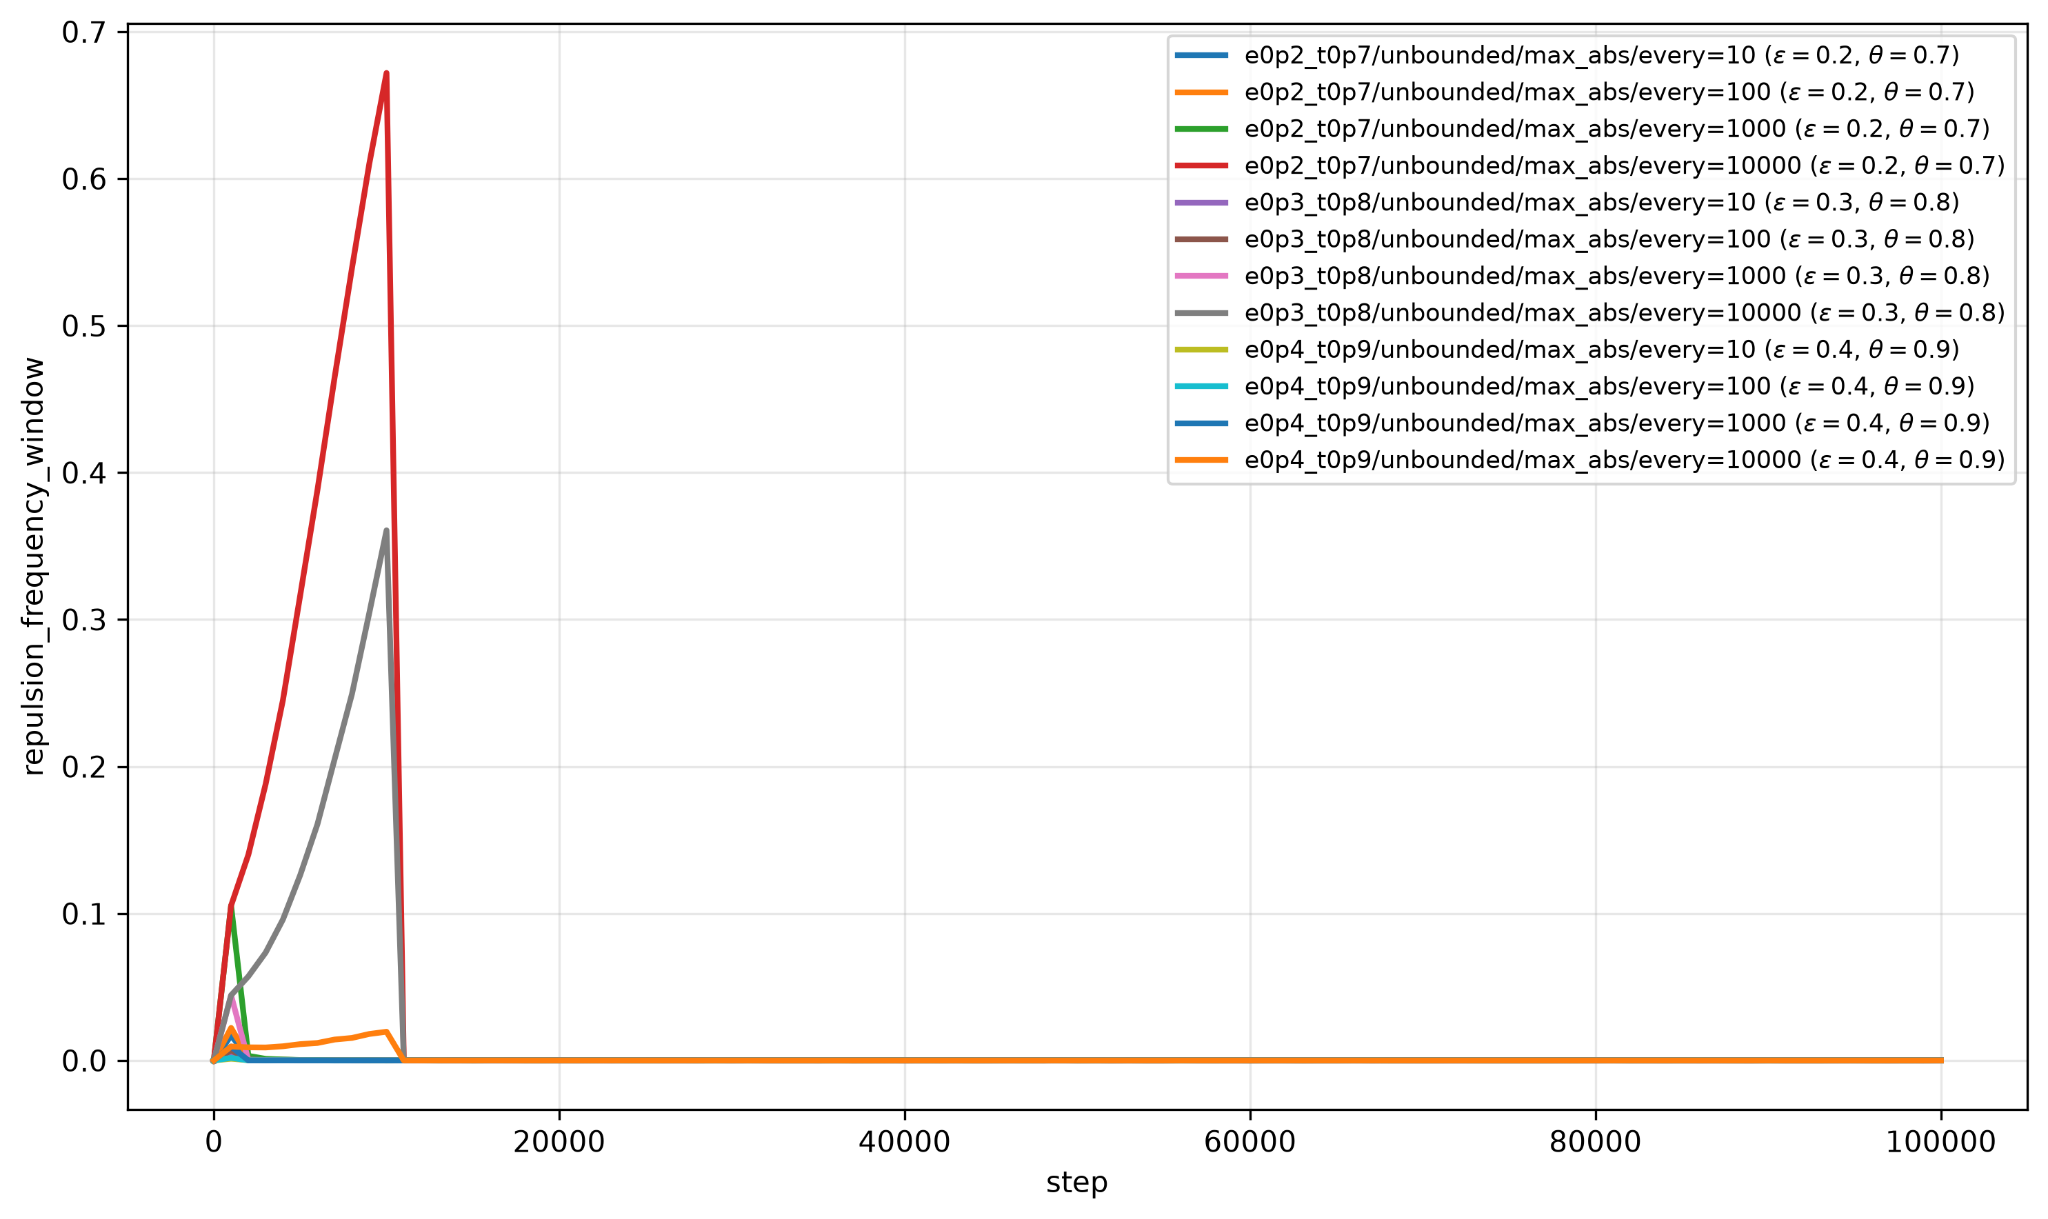
\includegraphics[width=\linewidth]{imagenes/experimento_4/repulsion_window.png}
  \caption{Frecuencia de repulsión.}
  \label{fig:exp04_repulsion}
\end{subfigure}
\caption{Evolución de las frecuencias de confianza y repulsión para diferentes umbrales y periodos de normalización $k$.}
\label{fig:exp04_interactions}
\end{figure}

La Figura~\ref{fig:exp04_interactions} muestra que, tras un momento concreto, las interacciones de repulsión se vuelven prácticamente nulas y la confianza pasa a dominar gran parte de las configuraciones. 

Sin embargo, el dominio de confianza no ocurre para todos las pruebas de normalización. En particular, para $(\epsilon,\theta)=(0.2,0.9)$ la frecuencia de confianza durante la etapa final pasa de aproximadamente $55.86\,\text{\%}$ con $k=10$ a $98.24\,\text{\%}$ con $k=10000$. En el primer caso, los casos restante corresponde principalmente a inacción y no a repulsión. Esto se debe a que los valores de la diferencia de las opiniones se quedan constantes entre el umbral de confianza y el umbral de repulsión.

\subsection{Resultados finales}

La Tabla~\ref{tab:exp04_selected} recoge la pruebas a los $100\,000$ pasos. La columna de confianza corresponde a la frecuencia media, la desviación típica y el número de clústeres son medias de los resultados finales de las $100$ ejecuciones.

\begin{table}[htbp]
\centering
\caption{Resultados finales seleccionados del ATBCR con normalización
\texttt{max\_abs}.}
\label{tab:exp04_selected}
\small
\begin{tabular}{ccrrr}
\toprule
$(\epsilon,\theta)$ & $k$ & Confianza (\%) & Desv. típica & Clústeres \\
\midrule
$(0.2,0.7)$ & 10    & 99.25 & 0.0445 & 5.14 \\
$(0.2,0.7)$ & 10000 & 97.67 & 0.0634 & 14.80 \\
$(0.2,0.9)$ & 10    & 55.86 & 0.3637 & 9.24 \\
$(0.2,0.9)$ & 10000 & 98.24 & 0.0638 & 9.71 \\
$(0.3,0.8)$ & 10    & 99.63 & 0.0385 & 2.97 \\
$(0.3,0.8)$ & 10000 & 99.23 & 0.0518 & 5.45 \\
$(0.4,0.9)$ & 10    & 99.70 & 0.0372 & 2.50 \\
$(0.4,0.9)$ & 10000 & 99.70 & 0.0362 & 2.43 \\
\bottomrule
\end{tabular}
\end{table}

Las diferencias en la dispersión y en el número de clústeres muestran que el periodo de normalización puede afectar a las opiniones finales. Para $(0.2,0.7)$, por ejemplo, la desviación típica media pasa de $0.0445$ con $k=10$ a $0.0634$ con $k=10000$, mientras que el número medio de clústeres aumenta de $5.14$ a $14.80$. La interpretación de los clústeres depende de la tolerancia que puse de $0.001$.

\subsection{Comparación de las distribuciones finales}

La Figura~\ref{fig:exp04_distributions} compara, para $(\epsilon,\theta)=(0.2,0.7)$, la distribución final del modelo acotado para comparar con las obtenidas mediante normalización periódica.

\begin{figure}[htbp]
\centering
\begin{subfigure}[t]{0.32\textwidth}
 \centering
 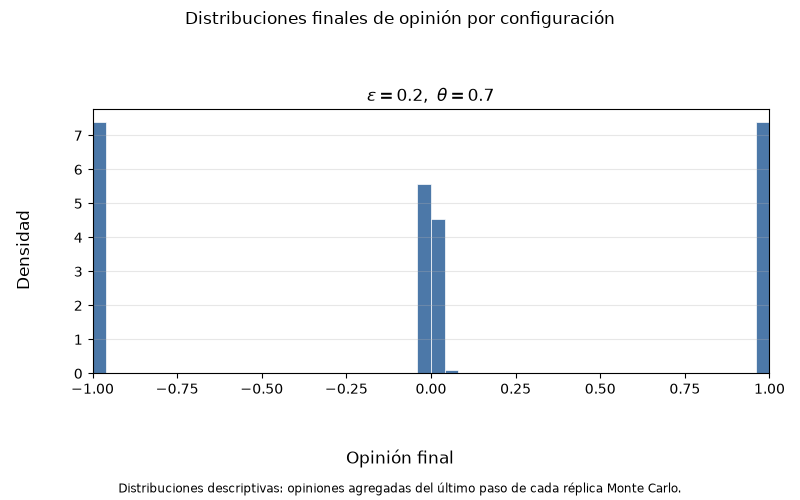
\includegraphics[width=\linewidth]{imagenes/experimento_4/bounded_reference.png}
 \caption{Referencia acotada.}
\end{subfigure}\hfill
\begin{subfigure}[t]{0.32\textwidth}
 \centering
 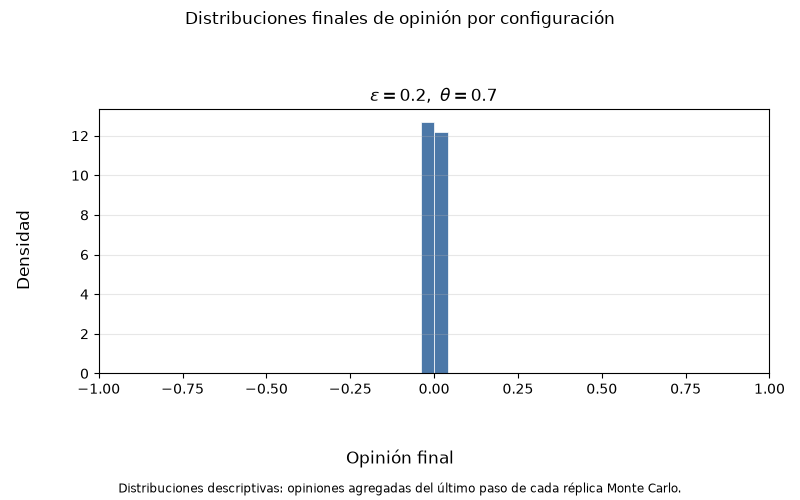
\includegraphics[width=\linewidth]{imagenes/experimento_4/maxabs_k10.png}
 \caption{Normalización cada 10 pasos.}
\end{subfigure}\hfill
\begin{subfigure}[t]{0.32\textwidth}
 \centering
 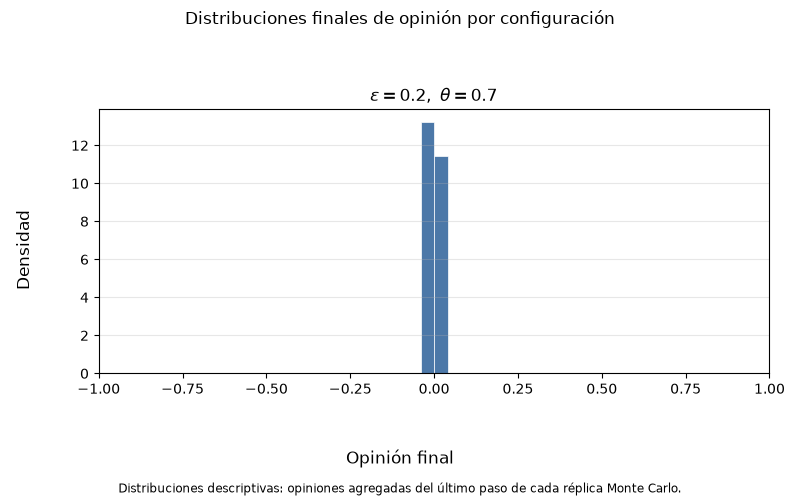
\includegraphics[width=\linewidth]{imagenes/experimento_4/maxabs_k10000.png}
 \caption{Normalización cada 10000 pasos.}
\end{subfigure}
\caption{Distribuciones de opinión al final de las simulaciones para $(\epsilon,\theta)=(0.2,0.7)$. Las tres gráficas utilizan el dominio $[-1,1]$.}
\label{fig:exp04_distributions}
\end{figure}

En el caso mostrado, la referencia acotada presenta opiniones en las regiones extremas y central, mientras que los casos normalizados existe una concentración más marcada alrededor del centro. Esta diferencia sugiere que la normalización no se limita a restringir las opiniones, sino que altera fuertemente la distribución de opiniones.

Aunque muchas configuraciones presentan frecuencias finales de confianza superiores al $99\,\text{\%}$, esta métrica solo indica que la mayor parte de las parejas seleccionadas cumplen el criterio de confianza. No demuestra que todos los agentes compartan la misma opinión ni que el estado se haya estabilizado temporalmente.

\subsection{Estabilidad temporal de las opiniones}
\label{subsec:exp04_estabilidad}

Para complementar el análisis previo, se estudia la estabilidad de las opiniones usando la normalización periódica \texttt{max\_abs}. En particular, se calcula el cambio máximo de opinión entre dos momentos consecutivos de una misma ejecución. Esta metrica mide la variación entre observaciones.

Se analiza el escenario $(\epsilon,\theta)=(0.2,0.7)$ para las frecuencias de normalización $k\in\{10,100,1000,10000\}$, utilizando la misma réplica Monte Carlo en las cuatro configuraciones.

\begin{figure}[htbp]
    \centering
  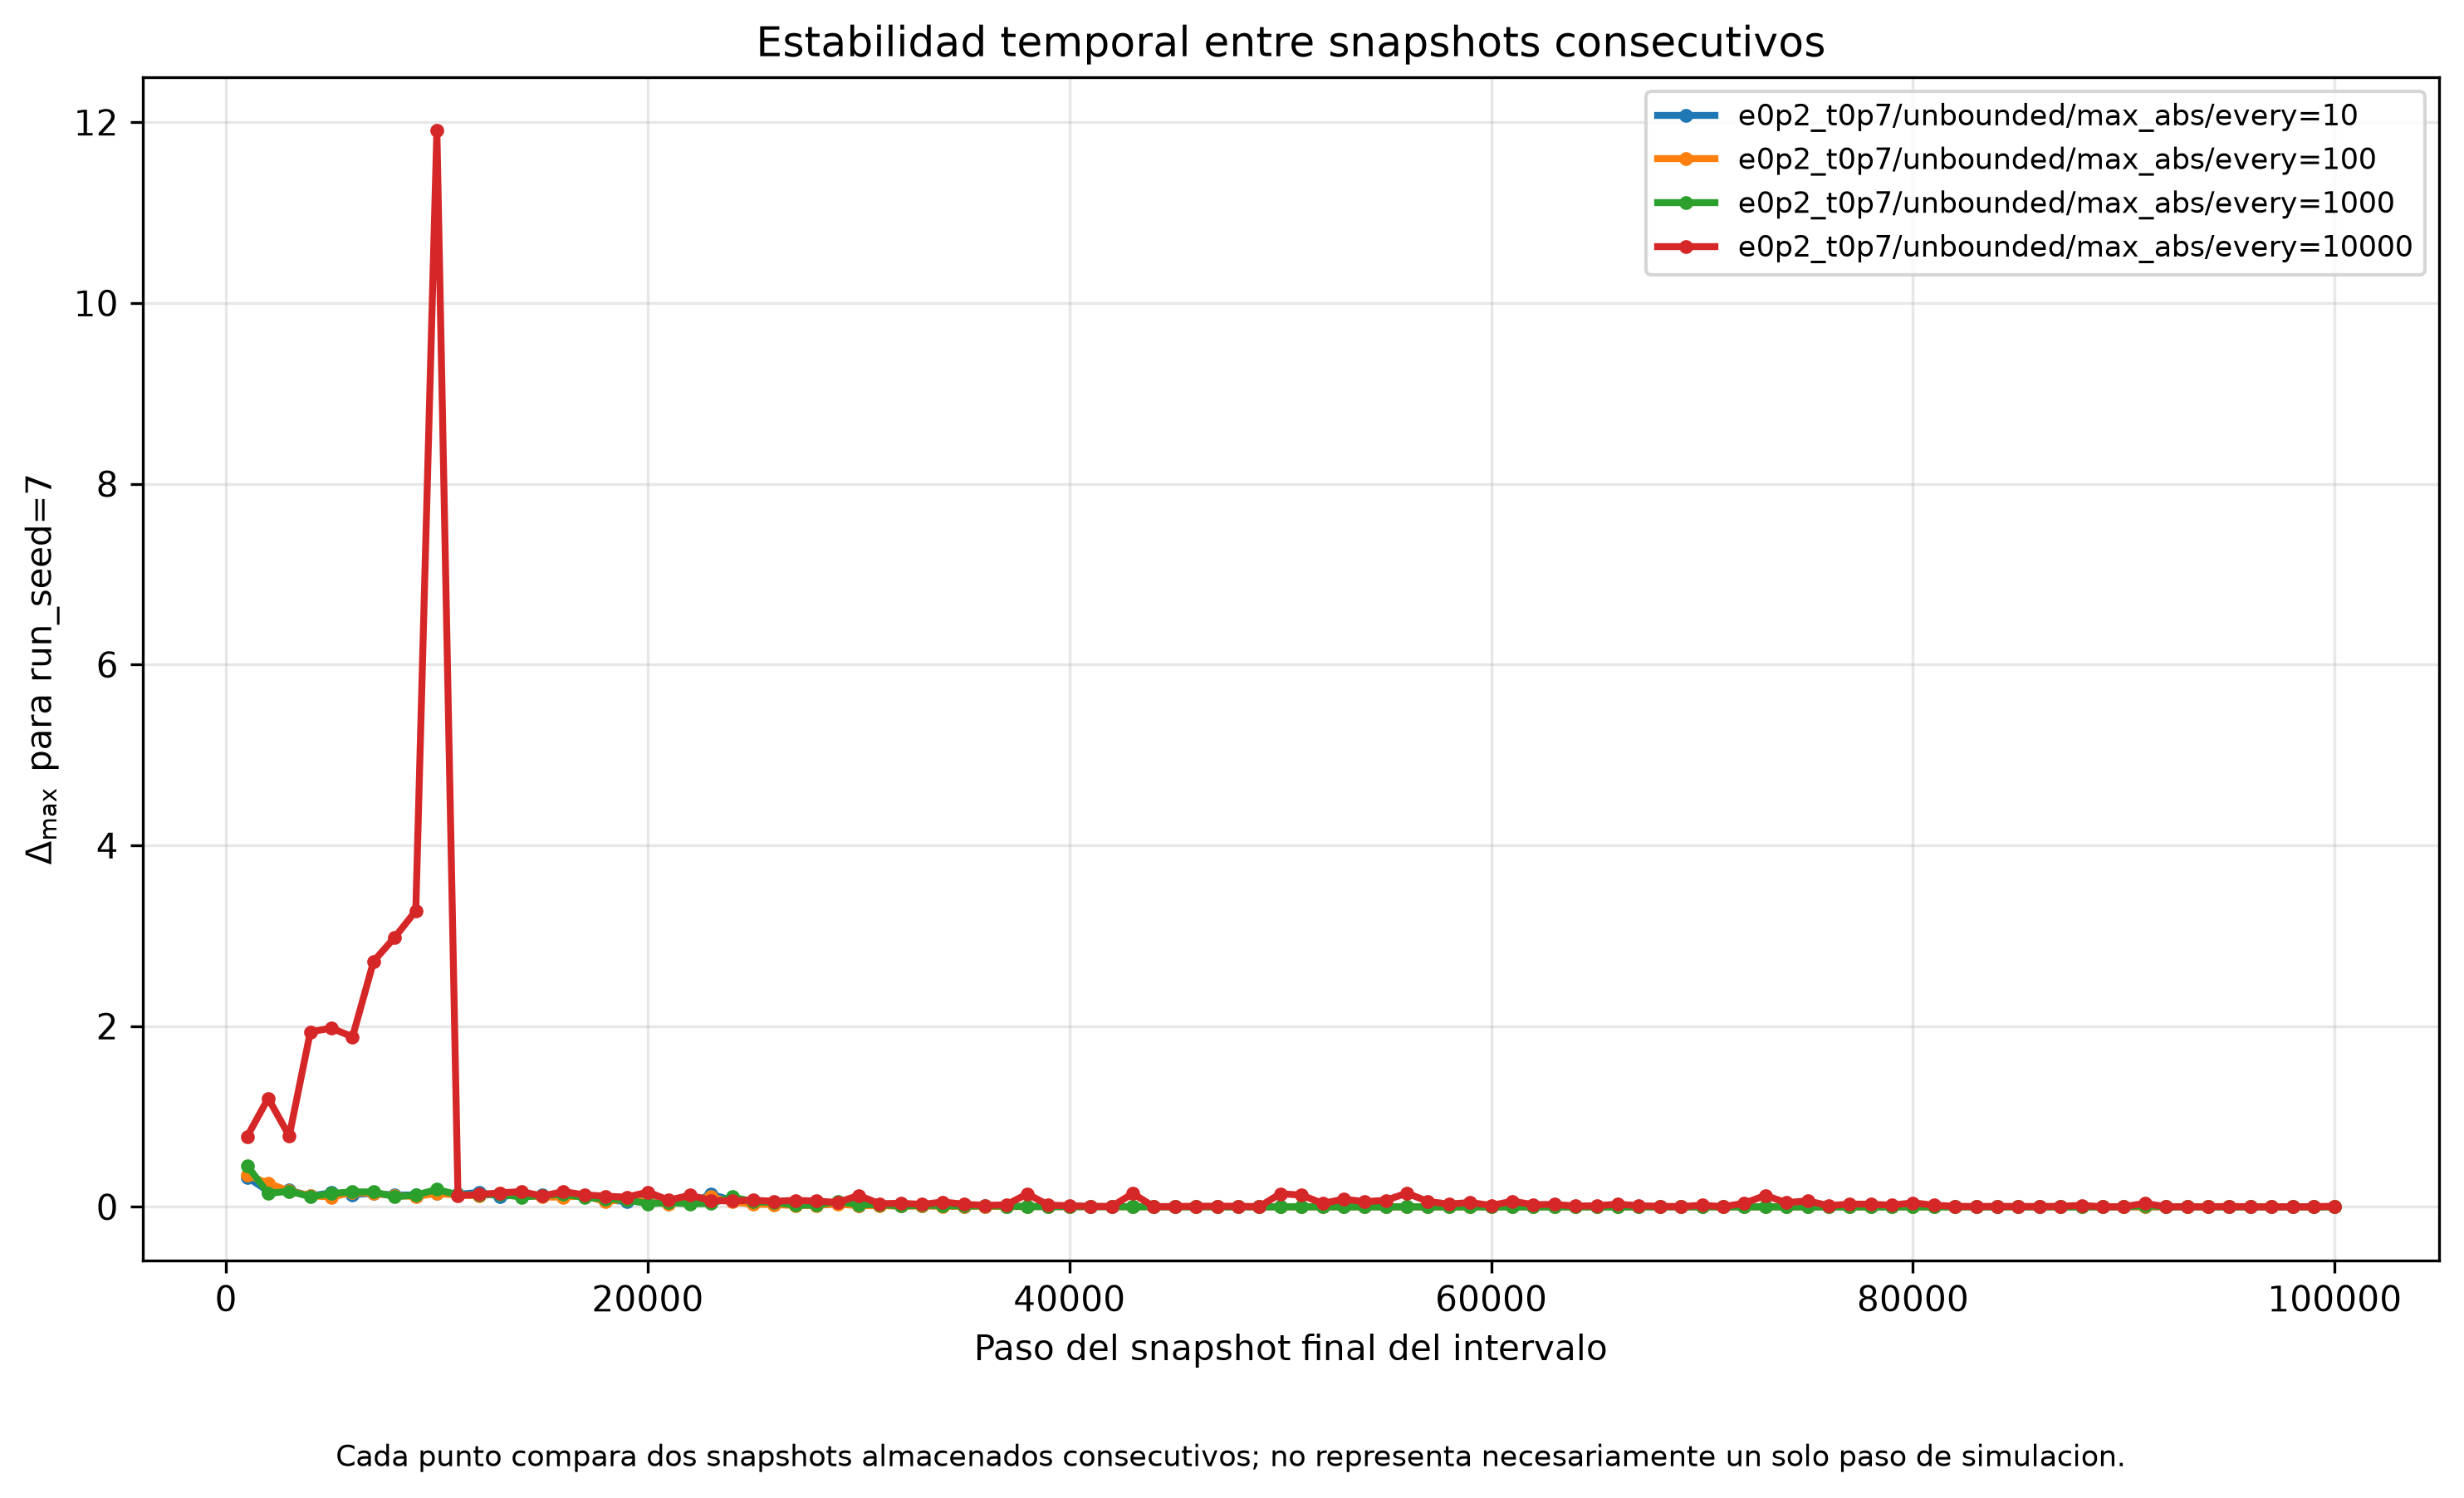
\includegraphics[width=0.95\linewidth]{imagenes/experimento_4/stability.png}
    \caption{Evolución del cambio máximo de opinión entre momentos consecutivos, para el escenario
    $(\epsilon,\theta)=(0.2,0.7)$ y diferentes periodos de normalización
    \texttt{max\_abs}.}
    \label{fig:exp04_estabilidad}
\end{figure}

En la Figura~\ref{fig:exp04_estabilidad}, al normalizar cada 10, 100 o 1000 pasos el cambio máximo entre estados registrados disminuye de forma progresiva. Para $k=10000$ se observa un crecimiento inicial distinto: las variaciones aumentan durante los primeros miles de pasos y presentan un pico alrededor de $t=10000$, coincidiendo con la primera normalización. Posteriormente, los cambios se reducen. Al final, las cuatro configuraciones muestran variaciones pequeñas entre observaciones, aunque persisten algunas fluctuaciones puntuales.

Estas observaciones aportan evidencia de una estabilización aproximada de los estados registrados. Sin embargo, no permiten demostrar convergencia estricta: las mediciones se realizan cada 1000 pasos y podrían ocultar cambios intermedios.




\subsection{Conclusiones del experimento}

La normalización periódica mediante \texttt{max\_abs} controla las opiniones en los instantes de normalización y evita que el crecimiento se mantenga. Sin embargo, este proceso de normalización afecta a las distancias absolutas entre agentes con respecto a umbrales fijo, por esto, modifica la distribución de los diferentes tipos de interacciones, en este caso la confianza suele dominar y la repulsión prácticamente desaparece al final.
El análisis entre momentos sugiere, una estabilización de las opiniones en la réplica examinada. No obstante, la normalización modifica las distancias a los umbrales fijos

Las distribuciones finales son diferentes de las del modelo acotado de referencia y dependen. Por tanto, \texttt{max\_abs} resulta útil como mecanismo de control de magnitudes, pero no constituye una transformación que mantenga la dinámica original del ATBCR.




\section{Experimento 0.5: normalización logarítmica con signo}
\label{sec:exp05}

\subsection{Objetivo}

El objetivo de este experimento es estudiar el comportamiento del modelo ATBCR cuando se aplica una normalización periódica basada en una transformación logarítmica con signo.

Esta propuesta surge como alternativa a la normalización lineal mediante máximo absoluto, estudiada en el Experimento 0.4, que mostró una concentración considerable de las opiniones alrededor de cero y una modificación del régimen de interacción respecto al modelo de referencia.

Se pretende determinar si una transformación no lineal permite controlar las magnitudes de opinión manteniendo una mayor separación entre los agentes y conservando mejor la estructura de las distribuciones finales.

\subsection{Formulación de la normalización}

Dado un conjunto de opiniones

\begin{equation}
    X(t)=\{x_1(t),x_2(t),\ldots,x_N(t)\},
\end{equation}

se aplica inicialmente una transformación logarítmica que conserva el signo de cada opinión:

\begin{equation}
    z_i(t)=
    \operatorname{sgn}(x_i(t))
    \ln(1+|x_i(t)|).
\end{equation}

La transformación permite operar sobre todo el dominio real, incluyendo opiniones negativas y el valor cero.

Posteriormente, se calcula el máximo absoluto de las opiniones transformadas:

\begin{equation}
    m_z(t)=\max_j |z_j(t)|.
\end{equation}

Finalmente, para $m_z(t)>0$, la normalización se define mediante:

\begin{equation}
    x_i^{\mathrm{norm}}(t)=
    \frac{z_i(t)}{m_z(t)}.
\end{equation}

En el caso degenerado $m_z(t)=0$, todas las opiniones transformadas son nulas y se mantiene el estado cero.

Esta operación garantiza que las opiniones normalizadas pertenecen al intervalo $[-1,1]$.

A diferencia de la normalización lineal, la transformación logarítmica comprime en mayor medida las magnitudes elevadas. Como consecuencia, las opiniones de menor magnitud pueden mantener una separación relativa mayor respecto a las opiniones extremas después de normalizar.

No obstante, esta transformación modifica las distancias absolutas entre agentes y, por tanto, puede alterar las reglas de interacción que se activan cuando los umbrales de confianza y repulsión permanecen constantes.

\subsection{Configuración experimental}

Se mantiene la configuración experimental utilizada en los experimentos anteriores:

\begin{itemize}
    \item Número de agentes: $N=1000$.
    \item Topología: grafo completo.
    \item Número de pasos: $T=100000$.
    \item Número de ejecuciones Monte Carlo:
          100 por configuración.
    \item Parámetro de actualización: $\mu=0.1$.
    \item Inicialización uniforme de las opiniones
          en $[-1,1]$.
    \item Evolución sin clipping entre normalizaciones.
    \item Frecuencias de normalización:
          $k\in\{10,100,1000,10000\}$.
\end{itemize}

Se consideran las nueve combinaciones de umbrales establecidas en el diseño experimental:

\begin{equation}
    \epsilon\in\{0.2,0.3,0.4\},
    \qquad
    \theta\in\{0.7,0.8,0.9\}.
\end{equation}

Siguiendo el criterio de los experimentos 0.2--0.4, los umbrales aplicados sobre el dominio $[-1,1]$ son los transformados:

\begin{equation}
    \epsilon'=2\epsilon,
    \qquad
    \theta'=2\theta.
\end{equation}

La normalización se aplica periódicamente después de ejecutar los correspondientes pasos de interacción.

\subsection{Evolución de las frecuencias de interacción}
\label{subsec:exp05_frecuencias}

Se analiza la evolución temporal de las frecuencias de confianza, inacción y repulsión utilizando ventanas temporales de 1000 pasos.

La Figura~\ref{fig:exp05_frequencies} muestra las frecuencias de confianza y repulsión para diferentes umbrales y periodos de normalización.

\begin{figure}[htbp]
    \centering

    \begin{subfigure}[b]{0.48\textwidth}
        \centering
        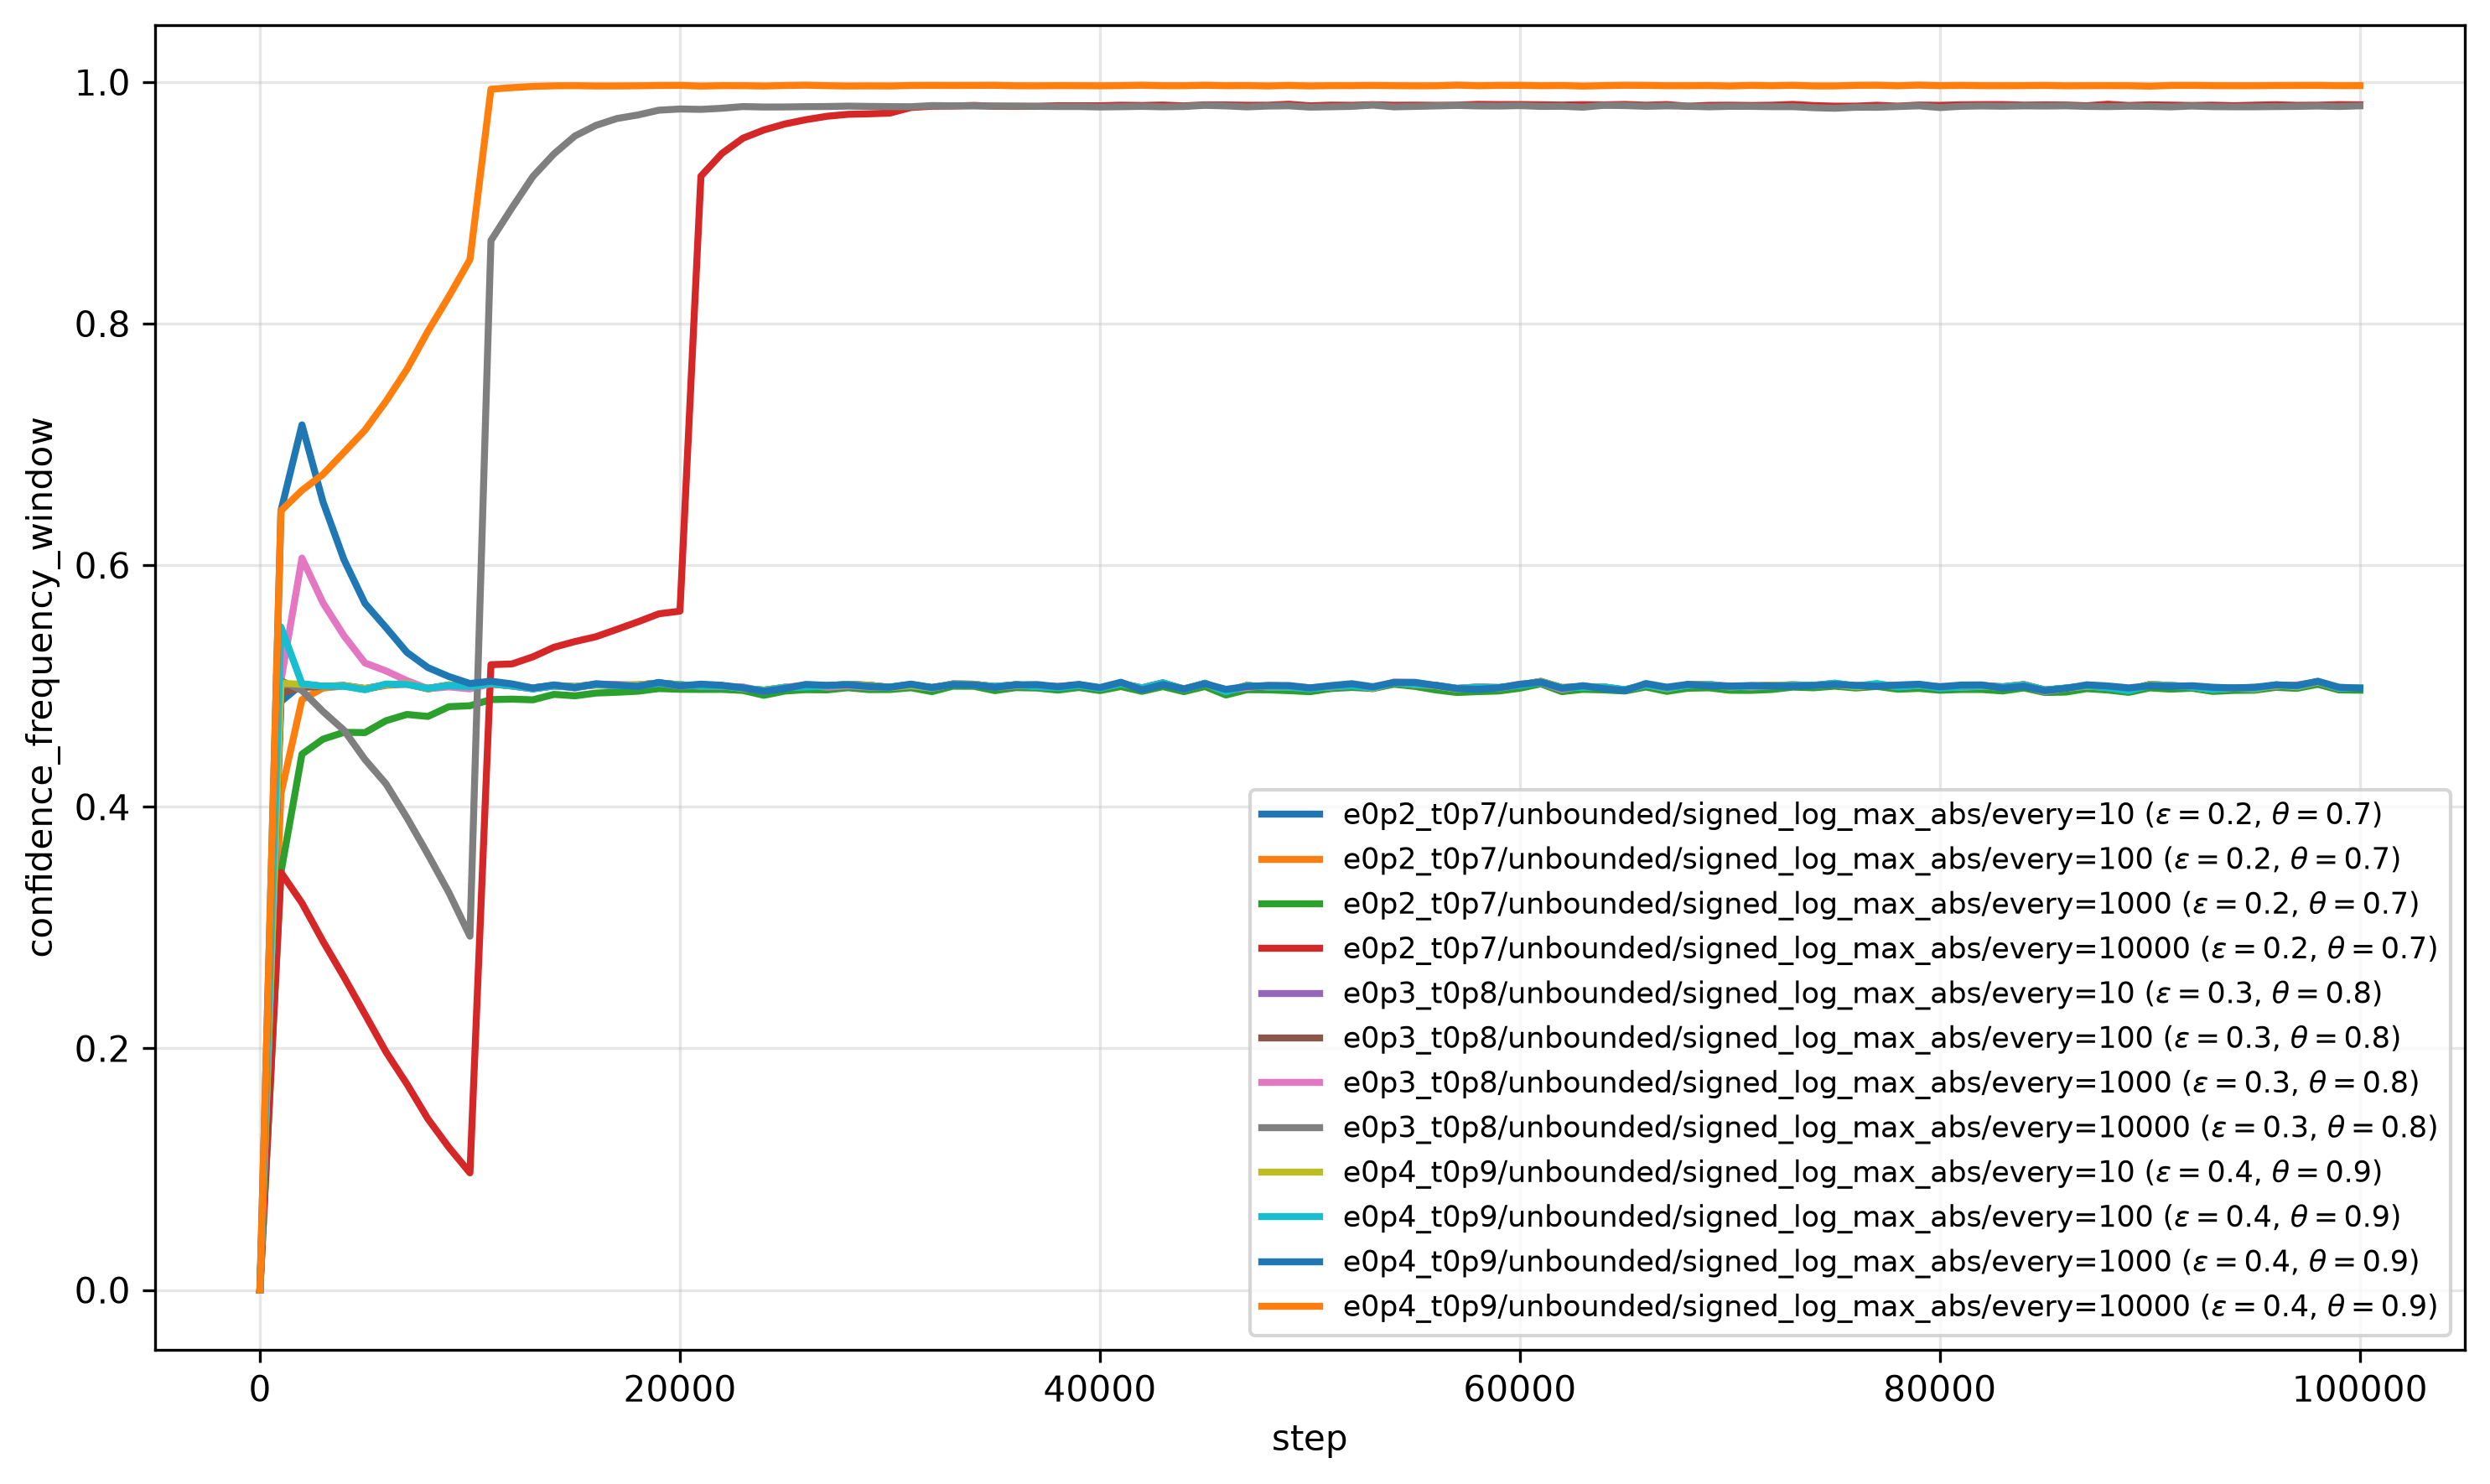
\includegraphics[width=\linewidth]{imagenes/experimento_5/confidence_compare_log.png}
        \caption{Frecuencia de confianza.}
        \label{fig:exp05_confidence}
    \end{subfigure}
    \hfill
    \begin{subfigure}[b]{0.48\textwidth}
        \centering
        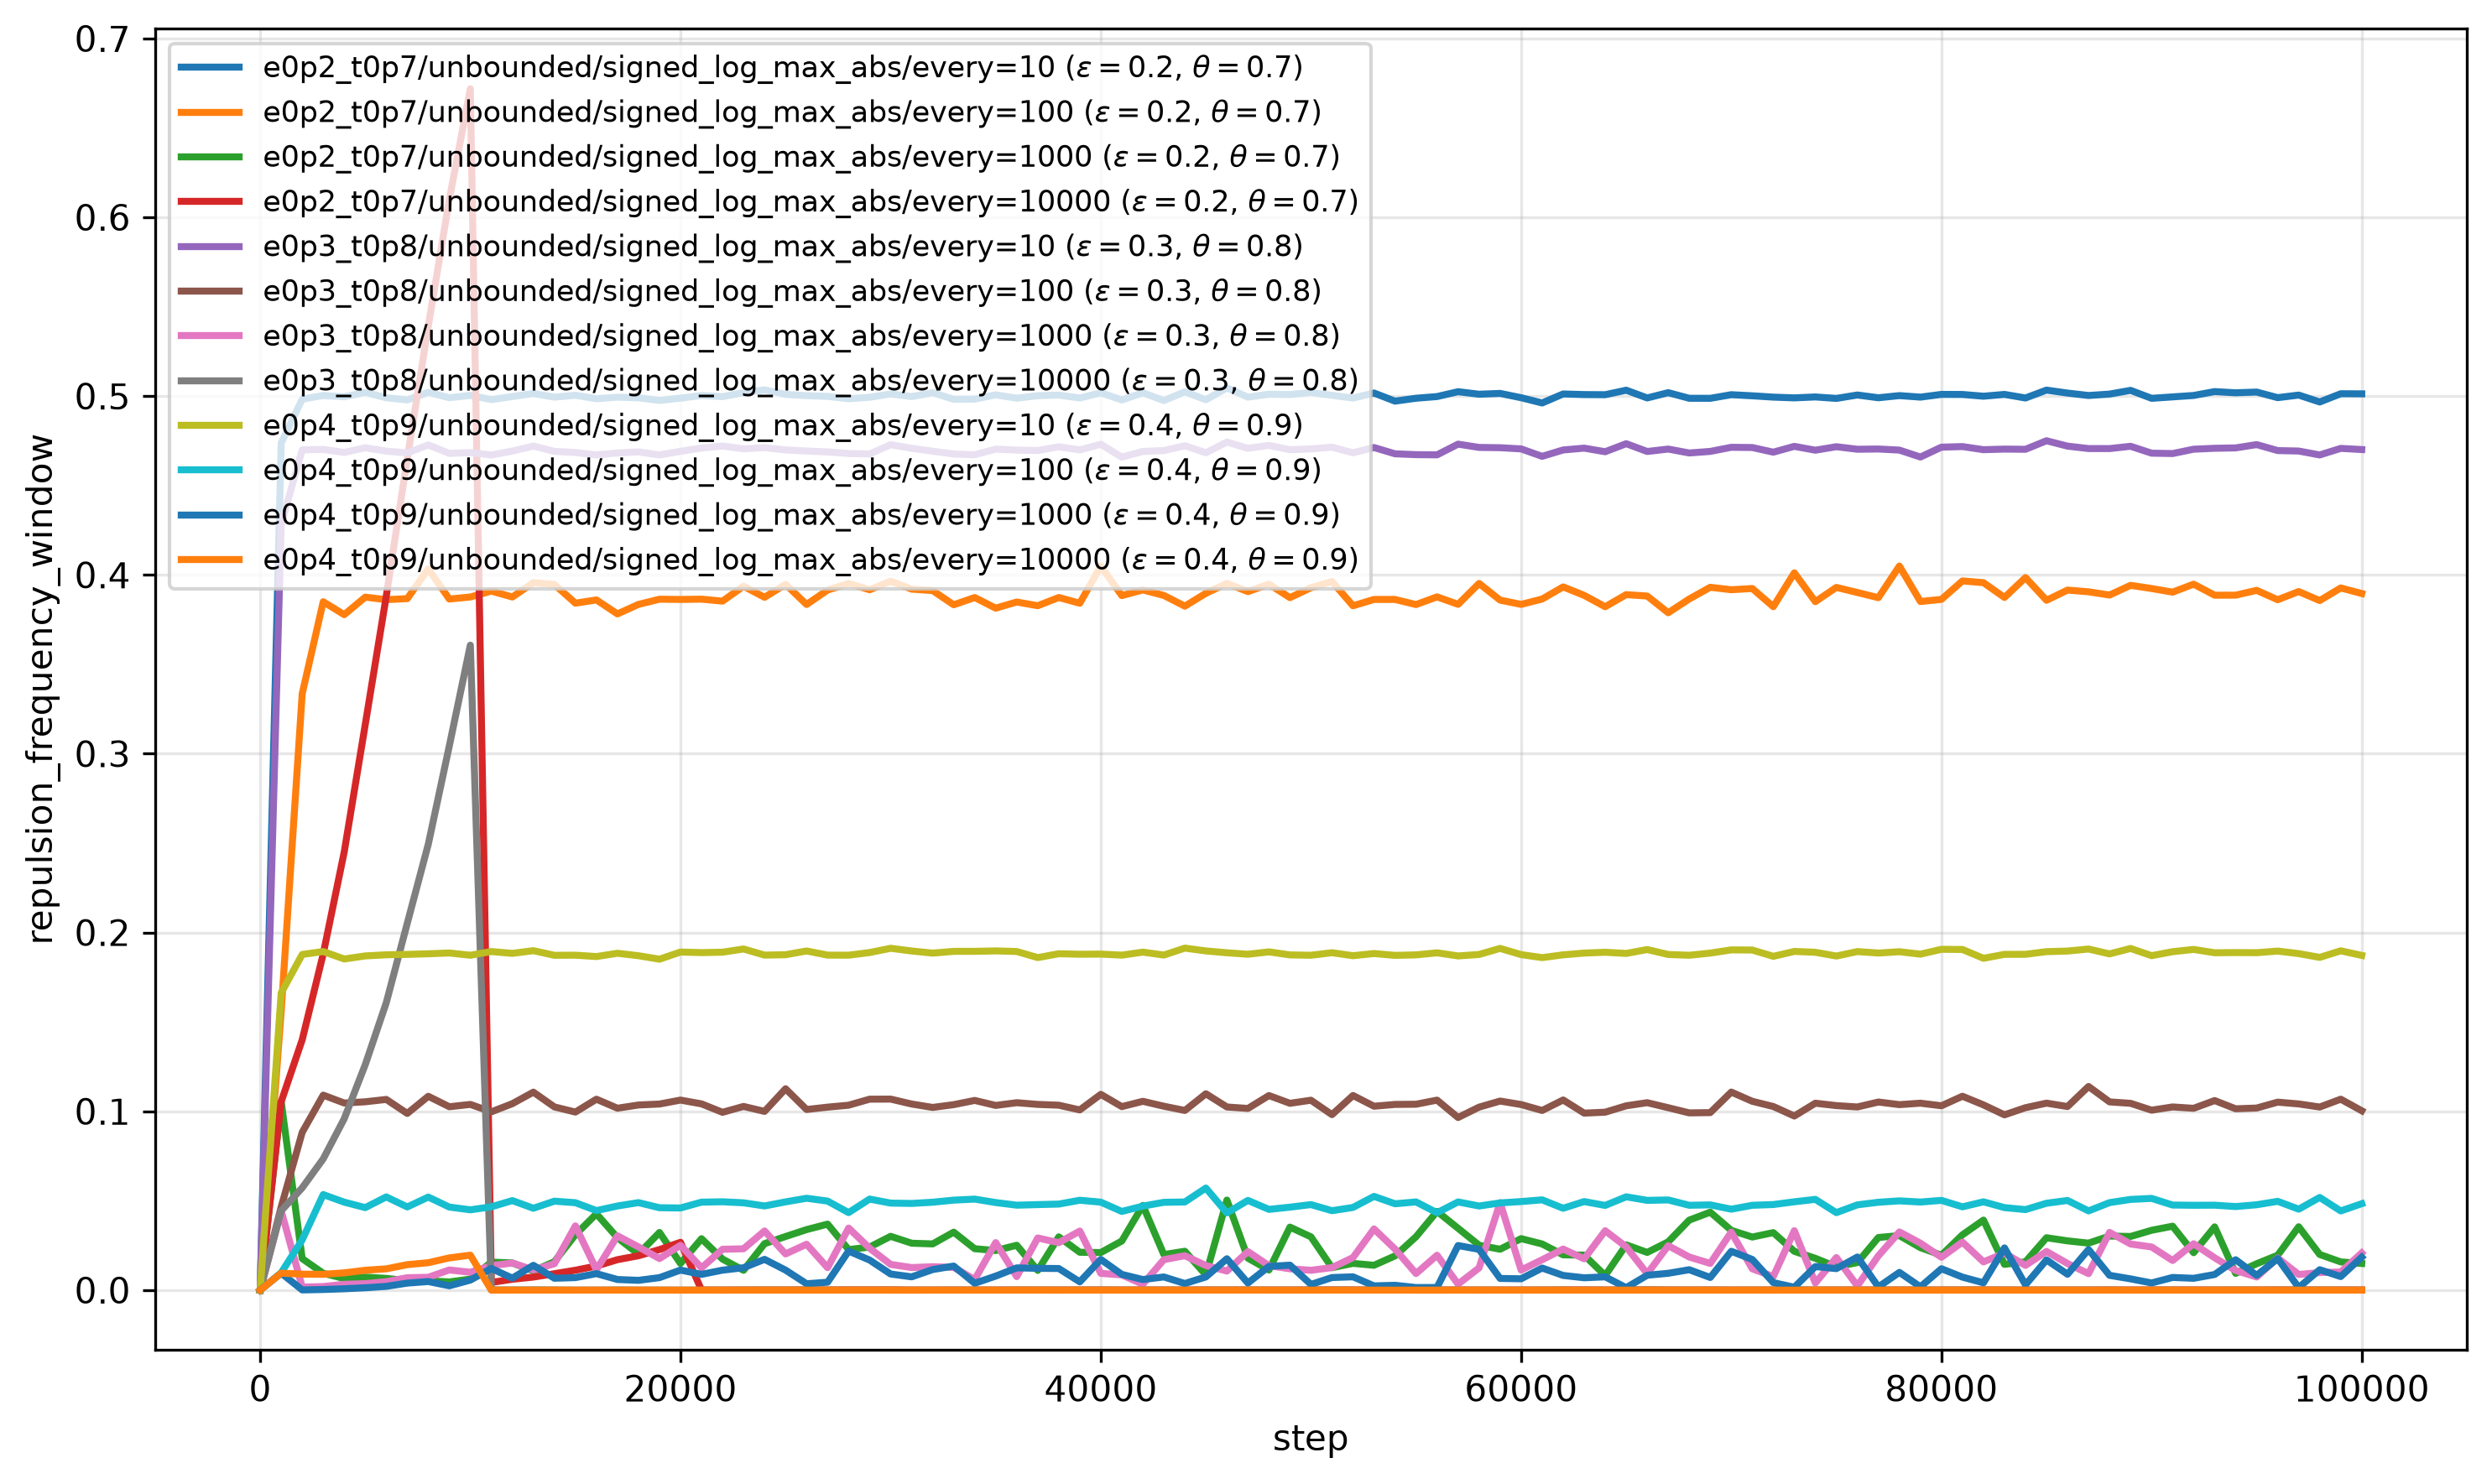
\includegraphics[width=\linewidth]{imagenes/experimento_5/repulsion_compare_log.png}
        \caption{Frecuencia de repulsión.}
        \label{fig:exp05_repulsion}
    \end{subfigure}

    \caption{Evolución temporal de las frecuencias de confianza y repulsión del ATBCR sin clipping con normalización logarítmica con signo. Las frecuencias corresponden a ventanas temporales de 1000 pasos y las curvas muestran los resultados agregados de las ejecuciones Monte Carlo.}
    \label{fig:exp05_frequencies}
\end{figure}

Los resultados muestran que la normalización logarítmica puede generar regímenes de interacción cualitativamente diferentes en función del intervalo de normalización y de los umbrales considerados.

Para normalizaciones frecuentes, se observan configuraciones en las que la confianza coexiste con una proporción importante de repulsión.

Sin embargo, al aumentar el intervalo entre normalizaciones, una parte de las interacciones repulsivas puede pasar al régimen de inacción, sin que ello suponga necesariamente un aumento equivalente de la frecuencia de confianza.

La Tabla~\ref{tab:exp05_interacciones} presenta un ejemplo correspondiente al escenario $(\epsilon,\theta)=(0.2,0.7)$ y a una ejecución con semilla 7.

\begin{table}[htbp]
    \centering
    \caption{Frecuencias de interacción en la última ventana temporal del Experimento 0.5 para el escenario $(\epsilon,\theta)=(0.2,0.7)$ y la ejecución con semilla 7.}
    \label{tab:exp05_interacciones}

    \begin{tabular}{rccc}
        \hline
        $k$ &
        Confianza (\%) &
        Inacción (\%) &
        Repulsión (\%) \\
        \hline
        10    & 48.8 & 0.8  & 50.4 \\
        100   & 48.7 & 10.2 & 41.1 \\
        1000  & 48.3 & 51.6 & 0.1 \\
        10000 & 97.8 & 2.2  & 0.0 \\
        \hline
    \end{tabular}
\end{table}

Este ejemplo muestra que reducir la frecuencia de normalización puede modificar sustancialmente la proporción de interacciones repulsivas y de inacción.

Asimismo, las configuraciones estudiadas evidencian que no existe una relación monótona sencilla entre la frecuencia de normalización y el predominio de las interacciones de confianza.

\subsection{Distribuciones finales de opinión}
\label{subsec:exp05_distribuciones}

Con el objetivo de evaluar la estructura final de las opiniones, se analizan los histogramas obtenidos al finalizar las simulaciones.

Se toma como caso representativo la configuración:

\begin{equation}
    (\epsilon,\theta)=(0.2,0.7).
\end{equation}

La Figura~\ref{fig:exp05_distributions} compara las distribuciones finales correspondientes a las cuatro frecuencias de normalización.

\begin{figure}[htbp]
    \centering
    \includefigureorplaceholder[width=0.95\textwidth]
    {figures/exp05_distributions.pdf}

    \caption{Distribuciones finales de opinión para $k\in\{10,100,1000,10000\}$ con normalización logarítmica con signo y $(\epsilon,\theta)=(0.2,0.7)$. Los histogramas representan las opiniones finales agregadas de las ejecuciones Monte Carlo.}
    \label{fig:exp05_distributions}
\end{figure}

Los resultados muestran una dependencia clara entre la frecuencia de normalización y la organización final de las opiniones.

Cuando la normalización se aplica cada 10 pasos, se observa una distribución fuertemente bimodal, con dos agrupaciones próximas a opiniones negativas y positivas de magnitud elevada.

Al aumentar el intervalo a 100 pasos, la distribución continúa siendo bimodal, aunque las agrupaciones aparecen ligeramente desplazadas hacia el centro y presentan una mayor dispersión.

Para normalizaciones cada 1000 pasos, siguen observándose dos agrupaciones diferenciadas, pero con opiniones de menor magnitud absoluta.

Finalmente, al normalizar cada 10000 pasos, la distribución presenta una concentración predominantemente central, sin la separación bimodal observada en las frecuencias anteriores.

Por tanto, la frecuencia de normalización influye tanto en las reglas de interacción como en las distribuciones finales del modelo.

\subsection{Análisis de ejecuciones individuales}
\label{subsec:exp05_individual}

Para comprobar si la bimodalidad observada era consecuencia de la agregación de múltiples simulaciones, se analizaron histogramas finales de tres ejecuciones Monte Carlo individuales.

Se utilizaron las semillas 7, 8 y 9 para el escenario $(\epsilon,\theta)=(0.2,0.7)$.

Los resultados muestran que, para frecuencias de normalización de 10, 100 y 1000 pasos, las ejecuciones inspeccionadas presentan dos agrupaciones diferenciadas de opinión.

Por tanto, la bimodalidad también aparece dentro de las simulaciones individuales estudiadas y no se debe exclusivamente a la agregación de réplicas.

Por el contrario, en las ejecuciones con normalización cada 10000 pasos se observa una concentración de las opiniones en una región central.

La Figura~\ref{fig:exp05_individual} recoge una comparación de estos resultados.

\begin{figure}[htbp]
    \centering
    \includefigureorplaceholder[width=0.95\textwidth]
    {figures/exp05_individual_distributions.pdf}

    \caption{Distribuciones finales de opiniones en ejecuciones Monte Carlo individuales del Experimento 0.5, comparando diferentes frecuencias de normalización. Se utilizan las semillas 7, 8 y 9.}
    \label{fig:exp05_individual}
\end{figure}

Esta comprobación permite interpretar con mayor precisión los histogramas agregados, aunque no constituye una clasificación exhaustiva de las 100 ejecuciones.

\subsection{Comparación con la normalización lineal}

Los resultados del Experimento 0.5 muestran diferencias significativas respecto a la normalización lineal del Experimento 0.4.

Mientras que la normalización mediante \texttt{max\_abs} favorece generalmente una concentración central de las opiniones, la normalización logarítmica con signo puede mantener dos agrupaciones polarizadas.

Asimismo, con \texttt{max\_abs} se observaron frecuencias elevadas de confianza en la mayoría de las configuraciones.

Por el contrario, \texttt{signed\_log\_max\_abs} permite que las interacciones de confianza coexistan con repulsión o inacción, dependiendo de los parámetros utilizados.

Sin embargo, la conservación de agrupaciones polarizadas no implica necesariamente una mejor reproducción del ATBCR acotado original.

En el escenario analizado, el modelo de referencia presenta simultáneamente agrupaciones centrales y extremas, mientras que la normalización logarítmica tiende a producir distribuciones bimodales o centrales, en función de la frecuencia de normalización.

\subsection{Conclusiones del Experimento 0.5}

La normalización logarítmica con signo constituye una alternativa a la normalización lineal para controlar las magnitudes de opinión en el ATBCR sin clipping.

Los resultados muestran que esta transformación permite mantener una mayor separación relativa entre determinados grupos de agentes, especialmente cuando se aplica con elevada frecuencia.

Sin embargo, la frecuencia de normalización condiciona considerablemente el régimen de interacción y la estructura final de las opiniones.

En particular, se han observado distribuciones polarizadas con normalizaciones frecuentes y una concentración central cuando el intervalo de normalización es mayor, en el escenario estudiado.

Por tanto, aunque la normalización logarítmica evita parte de la compresión central observada con la normalización lineal, no reproduce de forma consistente la estructura del modelo ATBCR acotado.

Los resultados indican que la transformación logarítmica debe considerarse una modificación de la dinámica del modelo y no una simple transformación de escala que conserve sus propiedades originales.



\section{Conclusiones generales}
\label{sec:paso0_conclusiones}

El objetivo del Paso 0 ha sido analizar diferentes modificaciones del modelo ATBCR con el propósito de estudiar su comportamiento fuera del dominio acotado original y evaluar mecanismos que permitan controlar las magnitudes de opinión.

Para ello, se realizaron cinco experimentos que permiten diferenciar el efecto del cambio de representación, la eliminación del clipping y la introducción de normalizaciones periódicas.

\subsection{Equivalencia entre dominios}

En primer lugar, el Experimento 0.1 permitió establecer una referencia experimental del modelo ATBCR original en el intervalo $[0,1]$.

Posteriormente, el Experimento 0.2 estudió la transformación afín:

\begin{equation}
    y_i(t)=2x_i(t)-1,
\end{equation}

que permite representar las opiniones en el intervalo $[-1,1]$.

Al transformar proporcionalmente los umbrales de confianza y repulsión, se comprobó que las trayectorias obtenidas conservaban el comportamiento del modelo original, salvo las diferencias numéricas inherentes a la representación en coma flotante.

Este resultado permitió disponer de un modelo de referencia en $[-1,1]$ para los experimentos posteriores.

\subsection{Consecuencias de eliminar el clipping}

En el Experimento 0.3 se eliminó la restricción del dominio de las opiniones, permitiendo que estas evolucionaran sobre el conjunto de los números reales.

Los resultados mostraron un crecimiento sostenido de las magnitudes de opinión durante el horizonte temporal analizado.

En las configuraciones estudiadas, la evolución de las magnitudes máximas fue compatible con un crecimiento aproximadamente exponencial.

Además, se observó un incremento progresivo de las frecuencias de interacción repulsiva, acompañado de una disminución de las interacciones de confianza.

Los umbrales de confianza y repulsión influyeron en el tiempo necesario para alcanzar el régimen dominado por repulsión, así como en la evolución de las magnitudes de opinión.

Sin embargo, los resultados obtenidos no constituyen una demostración matemática de divergencia para cualquier configuración o condición inicial.

\subsection{Efecto de la normalización lineal}

El Experimento 0.4 introdujo una normalización periódica basada en el máximo absoluto de las opiniones.

Esta estrategia permitió controlar las magnitudes en los instantes de normalización y reducir considerablemente la dispersión observada en el modelo sin clipping.

Asimismo, se observó un predominio de las interacciones de confianza en la mayoría de las configuraciones.

No obstante, las distribuciones finales presentaron una fuerte concentración central, diferente de la estructura obtenida con el modelo de referencia.

Por otra parte, el análisis del cambio máximo entre snapshots consecutivos mostró una reducción progresiva de las variaciones de opinión, lo que constituye evidencia de estabilización temporal aproximada.

Esta observación no implica necesariamente convergencia matemática ni consenso global.

\subsection{Efecto de la normalización logarítmica}

En el Experimento 0.5 se analizó una normalización logarítmica con signo, diseñada para reducir las magnitudes elevadas sin comprimir proporcionalmente todas las opiniones.

Los resultados mostraron que esta transformación genera regímenes dinámicos diferentes a los de la normalización lineal.

En particular, se observaron configuraciones con coexistencia de confianza, inacción y repulsión, así como distribuciones finales polarizadas.

La estructura de dichas distribuciones dependió de la frecuencia de normalización.

En el escenario analizado, las normalizaciones frecuentes generaron agrupaciones bimodales, mientras que las normalizaciones más espaciadas favorecieron una concentración central.

Las comprobaciones realizadas sobre ejecuciones individuales confirmaron que los grupos polarizados observados no eran exclusivamente consecuencia de agregar diferentes simulaciones.

Sin embargo, tampoco esta normalización reprodujo de forma consistente la distribución del ATBCR acotado original.

\subsection{Comparación de las propuestas}

Los resultados obtenidos permiten distinguir tres aspectos fundamentales:

\begin{enumerate}
    \item La transformación afín del dominio, acompañada de la adaptación correspondiente de los umbrales, conserva la dinámica del modelo de referencia.

    \item La eliminación del clipping puede conducir a un crecimiento sostenido de las magnitudes y a un régimen dominado por repulsión.

    \item Las normalizaciones periódicas controlan las magnitudes, pero también modifican las distancias entre agentes y, por tanto, las reglas de interacción del modelo.
\end{enumerate}

En consecuencia, la normalización no debe interpretarse únicamente como una operación numérica para mantener las opiniones dentro de un intervalo determinado.

Cuando los umbrales permanecen constantes, la modificación de las distancias puede provocar transiciones entre los regímenes de confianza, inacción y repulsión.

Por tanto, las normalizaciones estudiadas constituyen modificaciones efectivas de la dinámica del ATBCR.

\subsection{Implicaciones para el modelo propuesto}

El análisis desarrollado en el Paso 0 permite identificar varias propiedades relevantes para la construcción de futuras extensiones del ATBCR.

En primer lugar, resulta necesario distinguir entre controlar la magnitud de las opiniones y preservar la estructura de interacciones del modelo.

En segundo lugar, debe considerarse el efecto de cualquier transformación sobre las distancias entre agentes y su relación con los umbrales de confianza y repulsión.

Finalmente, la evaluación de nuevas propuestas no debería limitarse a verificar que las opiniones permanezcan acotadas, sino que también debe estudiar las distribuciones finales, los regímenes de interacción y la estabilidad temporal.

Los experimentos realizados proporcionan una base empírica para diseñar y comparar nuevas formulaciones del modelo, identificando las ventajas y limitaciones de los mecanismos de normalización estudiados.

\subsection{Conclusión final}

Los resultados del Paso 0 muestran que es posible controlar las magnitudes de opinión mediante normalizaciones periódicas, pero que este control puede alterar sustancialmente el comportamiento del modelo ATBCR.

La normalización lineal tiende a favorecer la concentración de opiniones, mientras que la normalización logarítmica con signo puede mantener agrupaciones polarizadas en determinadas configuraciones.

Ninguna de las dos alternativas ha demostrado conservar de forma general la estructura dinámica del modelo acotado original.

En consecuencia, el estudio pone de manifiesto la necesidad de considerar conjuntamente el dominio de las opiniones, las distancias entre agentes y los umbrales de interacción al desarrollar nuevas formulaciones de modelos de dinámica de opiniones.


\end{document}
